\documentclass[a4paper]{report}\usepackage[]{graphicx}\usepackage[]{color}
%% maxwidth is the original width if it is less than linewidth
%% otherwise use linewidth (to make sure the graphics do not exceed the margin)
\makeatletter
\def\maxwidth{ %
  \ifdim\Gin@nat@width>\linewidth
    \linewidth
  \else
    \Gin@nat@width
  \fi
}
\makeatother

\definecolor{fgcolor}{rgb}{0.345, 0.345, 0.345}
\newcommand{\hlnum}[1]{\textcolor[rgb]{0.686,0.059,0.569}{#1}}%
\newcommand{\hlstr}[1]{\textcolor[rgb]{0.192,0.494,0.8}{#1}}%
\newcommand{\hlcom}[1]{\textcolor[rgb]{0.678,0.584,0.686}{\textit{#1}}}%
\newcommand{\hlopt}[1]{\textcolor[rgb]{0,0,0}{#1}}%
\newcommand{\hlstd}[1]{\textcolor[rgb]{0.345,0.345,0.345}{#1}}%
\newcommand{\hlkwa}[1]{\textcolor[rgb]{0.161,0.373,0.58}{\textbf{#1}}}%
\newcommand{\hlkwb}[1]{\textcolor[rgb]{0.69,0.353,0.396}{#1}}%
\newcommand{\hlkwc}[1]{\textcolor[rgb]{0.333,0.667,0.333}{#1}}%
\newcommand{\hlkwd}[1]{\textcolor[rgb]{0.737,0.353,0.396}{\textbf{#1}}}%
\let\hlipl\hlkwb

\usepackage{framed}
\makeatletter
\newenvironment{kframe}{%
 \def\at@end@of@kframe{}%
 \ifinner\ifhmode%
  \def\at@end@of@kframe{\end{minipage}}%
  \begin{minipage}{\columnwidth}%
 \fi\fi%
 \def\FrameCommand##1{\hskip\@totalleftmargin \hskip-\fboxsep
 \colorbox{shadecolor}{##1}\hskip-\fboxsep
     % There is no \\@totalrightmargin, so:
     \hskip-\linewidth \hskip-\@totalleftmargin \hskip\columnwidth}%
 \MakeFramed {\advance\hsize-\width
   \@totalleftmargin\z@ \linewidth\hsize
   \@setminipage}}%
 {\par\unskip\endMakeFramed%
 \at@end@of@kframe}
\makeatother

\definecolor{shadecolor}{rgb}{.97, .97, .97}
\definecolor{messagecolor}{rgb}{0, 0, 0}
\definecolor{warningcolor}{rgb}{1, 0, 1}
\definecolor{errorcolor}{rgb}{1, 0, 0}
\newenvironment{knitrout}{}{} % an empty environment to be redefined in TeX

\usepackage{amsmath}
\usepackage{alltt}
\usepackage[fontsize=13pt]{scrextend}
\usepackage[utf8]{vietnam}
\usepackage{verbatim}
\usepackage{listings}



\makeatletter
\title{Ứng dụng, đánh giá, và so sánh một số mô hình phân loại trong phân loại khách hàng thẻ tín dụng}\let\Title\@title
\author{Nguyễn Đức Hiếu}\let\Author\@author
\makeatother
%%%%%%%%%%%%%%%%%%%%%%%%%
% TITLE PAGE FORMATTING %
%%%%%%%%%%%%%%%%%%%%%%%%%
\usepackage{afterpage}
\usepackage{xcolor}
\usepackage{graphicx}

%%%%%%%%%%%%%%%%%%%%%%%%
% PARAGRAPH FORMATTING %
%%%%%%%%%%%%%%%%%%%%%%%%
\usepackage{enumitem}
% Indent first paragraphs after each sections
\usepackage{indentfirst}

% Document formatting
\usepackage{mathptmx}
\renewcommand{\baselinestretch}{1.3}
\usepackage[a4paper]{geometry}
  \geometry{
  top=25mm,
  left=35mm,
  bottom=25mm,
  right=25mm
  }
%%%%%%%%%%%%%%%%%%%%%
% HEADER AND FOOTER %
%%%%%%%%%%%%%%%%%%%%%
\usepackage{etoolbox}
\patchcmd{\chapter}{\thispagestyle{plain}}{\thispagestyle{fancy}}{}{}
\usepackage{fancyhdr}
\pagestyle{fancy}
\fancyhf{}
\lhead{}
\chead{\normalsize Chuyên đề thực tập chuyên ngành Toán Kinh tế}
\rhead{}
\lfoot{}
\cfoot{\normalsize 11131371 - Nguyễn Đức Hiếu}
\rfoot{\normalsize Trang \thepage}
\renewcommand{\headrulewidth}{0.4pt}
\renewcommand{\footrulewidth}{0.4pt}
%%%%%%%%%%%%%%%%%%%%%%
% SECTION FORMATTING %
%%%%%%%%%%%%%%%%%%%%%%


\usepackage{titlesec}

\titleformat{\chapter}[display]
  {\centering\Large\bfseries}
  {\MakeUppercase{\chaptertitlename}  \thechapter}{1em}
  {\MakeUppercase}

\titleformat{name=\chapter,numberless}[display]
  {\normalfont\Large\bfseries\filcenter}{}{1ex}
  {\MakeUppercase}[\vspace{1ex}]

\titleformat{\section}[hang]
  {\bfseries}
  {\thesection}{1em}
  {\MakeUppercase}

\titleformat{\subsection}[hang]
  {\bfseries}
  {\thesubsection}{1em}
  {}

\titleformat{\subsubsection}[block]
  {}
  {\thesubsubsection}{1em}
  {}

\titleformat{\paragraph}[block]
  {\hspace{1em}}
  {\theparagraph}{1em}
  {}

% Appearance on table of contents
\usepackage{titletoc}
\titlecontents{chapter}% <section-type>
  [0pt]% <left>
  {\bfseries}% <above-code>
  {\color{blue}CHƯƠNG \thecontentslabel:\quad}% <numbered-entry-format>
  {}% <numberless-entry-format>
  {\titlerule*[1pc]{.}\contentspage}% <filler-page-format>



\renewcommand{\thechapter}{\Roman{chapter}}
\renewcommand{\thesection}{\arabic{chapter}.\arabic{section}}
\renewcommand{\theparagraph}{\alph{paragraph},}
\renewcommand{\thetable}{\arabic{chapter}.\arabic{table}}   
\renewcommand{\thefigure}{\arabic{chapter}.\arabic{figure}}
%%%%%%%%%%%%%%%%%%%%%%  
% FIGURES AND TABLES %
%%%%%%%%%%%%%%%%%%%%%%
\usepackage{graphicx}
\usepackage[section]{placeins}
\usepackage[justification=centering]{caption}

%%%%%%%%%%%%%%%%%%%
% TOC FORMATTING  %
%%%%%%%%%%%%%%%%%%%
% \usepackage{tocloft}
% \renewcommand{\cftchappresnum}{\MakeUppercase\chaptername\ }
% % \renewcommand{\cftchapaftersnum}{          }
% % \renewcommand{\cftchapaftersnumb}{\newline}
% \renewcommand{\cftchapdotsep}{\cftdotsep}
% Package hyperref should be loaded last, as it rewrites many commands.
% \usepackage{tocloft}
\usepackage[colorlinks=true, citecolor=blue, linkcolor=blue]{hyperref}
\usepackage[all]{hypcap}
% Customise for table of contents labeling
\setcounter{tocdepth}{4}
\setcounter{secnumdepth}{4}
%%%%%%%%%%%%
% CITATION %
%%%%%%%%%%%%
% Setting up for citation styles
% \usepackage{natbib}
\usepackage[backend=bibtex,bibstyle=luanan,sorting=ydnt,style=authoryear]{biblatex}
\addbibresource{reference.bib}
% Add number to bibliography
\defbibenvironment{bibliography}
  {\enumerate
     {}
     {\setlength{\leftmargin}{\bibhang}%
      \setlength{\itemindent}{-\leftmargin}%
      \setlength{\itemsep}{\bibitemsep}%
      \setlength{\parsep}{\bibparsep}}}
  {\endenumerate}
  {\item}
%%%%%%%%%%%%%%%%%%%%%%%%%%%%%%%%%%%%%%%%%%%%
%%%%%%%%%%%%%%%%%%%%%%%%%%%%%%%%%%%%%%%%%%%%
%%%%---------DOCUMENT CONTENTS----------%%%%
%%%%%%%%%%%%%%%%%%%%%%%%%%%%%%%%%%%%%%%%%%%%
%%%%%%%%%%%%%%%%%%%%%%%%%%%%%%%%%%%%%%%%%%%%
\IfFileExists{upquote.sty}{\usepackage{upquote}}{}
\begin{document}
%%%%%%%%%%%%%%%%%%%%%%%%%%%%%%%
%         TITLE PAGE          %
%%%%%%%%%%%%%%%%%%%%%%%%%%%%%%%

\begin{titlepage}

\definecolor{titlepagecolor}{RGB}{1, 81, 159 }
% \definecolor{titlepagecolor}{RGB}{128, 0, 0 }
\color{white}
\pagecolor{titlepagecolor}\afterpage{\nopagecolor}
\large
\centering
\textbf{TRƯỜNG ĐẠI HỌC KINH TẾ QUỐC DÂN}

\textbf{KHOA TOÁN KINH TẾ}
\vspace{5mm}


\includegraphics[width=0.4\textwidth]{./Cover/neu-logo.png}\par\vspace{1cm}
{\bfseries\scshape\Huge Chuyên đề thực tập}


\begin{description}[leftmargin=6cm,style=nextline]
\item[Chuyên ngành:] Toán Kinh tế
\item[Đề tài:] \Title
\item[Sinh viên thực hiện:] Nguyễn Đức Hiếu
\item[Mã sinh viên:] 11131371
\item[Lớp:] Toán Kinh tế 55
\item[Giảng viên hướng dẫn:] PGS. Nguyễn Thị Minh
\end{description}

\centering
\vfill
% Bottom of the page
\makebox[0pt]{\rule{0.5\textwidth}{1pt}}

{\large Hà Nội,  \today\par}
\end{titlepage}


%%%%%%%
% TOC %
%%%%%%%
\pagenumbering{roman}

\addcontentsline{toc}{chapter}{Mục lục}
\clearpage\tableofcontents

\listoffigures
\addcontentsline{toc}{chapter}{Danh sách hình minh họa}

\begingroup
\let\clearpage\relax
\addcontentsline{toc}{chapter}{Danh sách bảng}
\listoftables
\endgroup




%%%%%%%%%%%%%%%
% Lời mở đầu %
%%%%%%%%%%%%%%%
\chapter*{Lời mở đầu}
\pagenumbering{arabic}
\addcontentsline{toc}{chapter}{Lời mở đầu}

% LỜI MỞ ĐẦU  
%
% - Nêu vấn đề
Đối với các ngân hàng việc chấm điểm tín dụng và phân loại các khách hàng là một trong những khâu thiết yếu cho quy trình quản trị rủi ro của ngân hàng.
%
Phương pháp truyền thống của việc ra quyết định có cho một cá nhân cụ thể vay hay không là dựa trên đánh giá cảm tính dựa trên kinh nghiệm cá nhân.
%
Tuy nhiên, sự phát triển về quy mô của nền kinh tế đã tạo ra sức ép về nhu cầu vay, đi kèm với đó là sự cạnh tranh giữa các ngân hàng và công nghệ máy tính ngày càng phát triển đã khiến cho việc sử dụng các mô hình thống kê trong việc phân loại các khách hàng tín dụng là bắt buộc đối với các ngân hàng trên thế giới mà ở Việt Nam cũng không phải là ngoại lệ.
%

Vậy, phương pháp ước lượng nào có thể giúp chúng ta xây dựng được hệ thống chấm điểm tín dụng chính xác nhất? Đã có một số nghiên cứu mang tính chất so sánh hiệu năng giữa các mô hình \parencite{baesens2003benchmarking, xiao2006comparative, lessmann2015benchmarking}. 
Sự khác biệt về hiệu năng của các phương pháp khác nhau là có, tuy nhiên hầu như là không đáng kể, và không phải các mô hình hiệu quả hơn đều là các mô hình mới và tân tiến.
Theo \textcite{thomas2010consumer}, cách hiệu quả để xây dựng một hệ thống lượng định hiệu quả là phối hợp nhiều mô hình khác nhau thay vì tìm kiếm một mô hình toàn diện có thể áp dụng với tất cả các ngân hàng.

Trong bài này, chúng ta sẽ tiếp cận đến một số phương pháp phân loại các khách hàng tín dụng phổ biến hiện nay và rút ra một số kết luận về việc sử dụng các phương pháp khác nhau sao cho hợp lý. Bài viết này được bố cục như sau:

\begin{itemize}
\item \textbf{Chương 1} đưa ra một cái nhìn tổng quan về lĩnh vực quản trị rủi ro tín dụng trong ngân hàng và đưa ra một số vấn đề của việc chấm điểm tín dụng tại các ngân hàng Việt Nam.
\item Các mô hình được thực hiện trong bài này sẽ được giới thiệu ở \textbf{Chương 2}, đi kèm với đó là một số chỉ tiêu sẽ được dùng để đánh giá mô hình trong bài này.
\item Trong \textbf{Chương 3}, chúng ta sẽ ứng dụng các phương pháp được giới thiệu ở \textbf{Chương 2} trong một bộ số liệu mẫu về các khách hàng thẻ tín dụng trong một ngân hàng ở Đài Loan.
\item Kết quả của các mô hình sẽ được thảo luận ở \textbf{Chương 4}, cùng với một số kết luận rút ra được sau khi áp dụng mô hình.
\end{itemize}

% - Hướng tiếp cận 
Đề tài này được soạn thảo bằng \LaTeX{} kết hợp với \texttt{Sweave} và \texttt{knitr} 
\parencite{r:knitr}. Tất cả phân tích được thực hiện trên phần mềm thống kê 
R version 3.4.0 (2017-04-21) \parencite{r:rbase},  
các phân tích cụ thể được thực hiện sử dụng các gói mở rộng \texttt{caret}\parencite{r:caret}, \texttt{tidyverse} \parencite{r:tidyverse}... Mô hình logit được thực hiện với gói \texttt{glmnet}\parencite{r:glmnet}. 
Mô hình SVM được thực hiện với gói \texttt{kernlab} \parencite{r:kernlab}, là một giao diện của phần mềm \texttt{LIBSVM} \parencite{CC01a} trong môi trường \texttt{R}.

%  Cảm ơn bla bla
Em xin cảm ơn giáo viên hướng dẫn, cô Nguyễn Thị Minh, cùng với các thầy cô giáo khác trong khoa đã tạo điều kiện cho em thực hiện đề tài này.


%%%%%%%%%%%%
% Chương 1 %
%%%%%%%%%%%%
\chapter{Tổng quan về quản trị rủi ro tín dụng đối với khách hàng cá nhân}
\section{Tổng quan về rủi ro tín dụng và vấn đề quản trị rủi ro trong ngân hàng}
\subsection{Khái niệm về rủi ro và chấm điểm tín dụng}
\subsubsection{Khái niệm rủi ro tín dụng}
\paragraph{Rủi ro}
% Nhiều quan niệm rủi ro 
Có nhiều cách quan niệm khác nhau về rủi ro phụ thuộc vào lĩnh vực mà nó áp dụng.  Tuy nhiên, các quan niệm đó  coi rủi ro là các biến cố không mong đợi, gây ra thiệt hại và có thể đo lường được.

% Quan niệm trong NHTM
Trong các ngân hàng thương mại, rủi ro được hiểu là những biến cố có thể gây ra thiệt hại cho lợi nhuận hay thậm chí là nguy cơ phá sản của các ngân hàng.

% Tầm quan trọng
Trong hoạt động kinh tế nói chung và trong hoạt động Ngân hàng nói riêng thì vấn đề rủi ro là không thể tránh khỏi. Vì thế, các ngân hàng  không thể loại bỏ được rủi ro mà chỉ có thể phát hiện kịp thời để có những biện pháp chủ động xử lý.

\paragraph{Rủi ro tín dụng}
Là rủi ro do một khách hàng hay một nhóm khách hàng vay vốn không trả được nợ cho Ngân hàng. Trong kinh doanh Ngân hàng, rủi ro tín dụng là loại rủi ro lớn nhất, thường xuyên xảy ra và gây hậu quả nặng nề có khi dẫn đến phá sản Ngân hàng.

Ngày nay, nhu cầu về vốn để mở rộng sản xuất kinh doanh, cải tiến trang thiết bị kỹ thuật, nâng cao công nghệ và các nhu cầu phục vụ sản xuất kinh doanh luôn tăng lên. Để đáp ứng nhu cầu này, các NHTM cũng phải luôn mở rộng quy mô hoạt động tín dụng, điêu đó có nghĩa là rủi ro tín dụng cũng phát sinh nhiều hơn.

Rủi ro tín dụng là loại rủi ro phức tạp nhất, việc quản lý và phòng ngừa nó rất khó khăn, nó có thể xảy ra ở bất cứ đâu, bất cứ lúc nào... Rủi ro tín dụng nếu không được phát hiện và sử lý kịp thời sẽ nảy sinh các rủi ro khác.

Rủi ro tín dụng có thể rơi vào một trong các loại sau:
\begin{itemize}
\item Rủi ro vỡ nợ: Rủi ro của các khoản thiệt hại phát sinh từ người đi vay không có khả năng thanh toán đầy đủ khoản nợ hoặc đã quá thời hạn quy định mà không có khả năng trả nợ. Rủi ro vỡ nợ có thể tác động đến tất cả các giao dịch nhạy cảm với tín dụng bao gồm các khoản vay, chứng khoán và các công cụ phái sinh.
\item Rủi ro tập trung: Rủi ro này xuất hiện khi ngân hàng thương mại cho vay một khách hàng hoặc một nhóm khách hàng có liên quan với mức tín dụng quá lớn so với năng lực tài chính của NHTM đó tại một thời điểm. Khi khách hàng gặp rủi ro trong hoạt động và không thể thanh toán nợ đúng hạn, NHTM cho vay có thể gặp vấn đề thanh khoản.
\item Rủi ro quốc gia Rủi ro khi những thay đổi kinh tế hay chính trị tại nước ngoài, ví dụ như thiếu dự trữ tiền tệ (hối đoái), sẽ gây chậm trễ thanh toán tiền vay cho các  ngân hàng tín dụng, cơ quan kiểm soát ngoại hối hoặc gây mất khoản nợ. Rủi ro thuộc về quốc gia có phạm vi rộng hơn rủi ro chủ quyền, vì nó xem xét suất hoàn trả nợ từ nhũng người vay tư nhân cũng như chính phủ trung ương. Các ngân hàng dành riêng các quỹ trong một tài khoản dự trữ, gọi là dự trữ rủi ro chuyển giao được phân bố, làm khoản đệm đối phó với những khoản lỗi nợ khó đòi có thể xảy ra từ các khoản vay nước ngoài.
\end{itemize}

\subsubsection{Nguyên nhân dẫn đến rủi ro tín dụng}
Thực tế kinh doanh của Ngân hàng trong thời gian qua cho thấy rủi ro tín dụng xảy ra là do những nguyên nhân sau:

\paragraph{Nguyên nhân từ phía Ngân hàng}
\begin{itemize}
\item Ngay hàng đưa ra chính sách tín dụng không phù hợp với nền kinh tế và thể lệ cho vay còn sơ hở để khách hàng lợi dụng chiếm đoạt vốn của Ngân hàng.
\item Do cán bộ Ngân hàng chưa chấp hành đúng quy trình cho vay như: không đánh giá đầy đủ chính xác khách hàng trước khi cho vay, cho vay khống, thiếu tài sản đảm bảo, cho vay vượt tỷ lệ an toàn. Đồng thời cán bộ Ngân hàng không kiểm tra, giám sát chặt chẽ về tình hình sử dụng vốn vay của khách hàng.
\item Do trình độ nghiệp vụ của cán bộ tín dụng còn nên việc đánh giá các dự án, hồ sơ xin vay còn chưa tốt, còn xảy ra tình trạng dự án thiếu tính khả thi mà vẫn cho vay.
\item Cán bộ Ngân hàng còn thiếu tinh thần trách nhiệm, vi phạm đạo đức kinh doanh như: thông đồng với khách hàng lập hồ sơ giả để vay vốn, xâm tiêu khi giải ngân hay thu nợ, đôi khi còn nể nang trong quan hệ khách hàng.
\item Ngân hàng đôi khi quá chú trọng về lợi nhuận, đặt những khoản vay có lợi nhuân cao hơn những khoản vay lành mạnh.
\item Do áp lực cạnh tranh với các Ngân hàng khác.
\item Do tình trạng tham nhũng, tiêu cực diễn ra trong nội bộ Ngân hàng
\end{itemize}

\paragraph{Nguyên nhân từ phía khách hàng.}

\begin{itemize}
\item Người vay vốn sử dụng vốn vay sai mục đích, sử dụng vào các hoạt động có rủi ro cao dẫn đến thua lỗ không trả được nợ cho Ngân hàng.
\item Do trình độ kinh doanh yếu kếm, khả năng tổ chức điều hành sản xuất kinh doanh của lãnh đạo còn hạn chế.
\item Doanh nghiệp vay ngắn hạn để đầu tư vào tài sản lưu động và cố định.
\item Doanh nghiệp sản xuất kinh doanh thiếu sự linh hoạt, không cải tiến quy trình công nghệ, không trang bị máy móc hiện đại, không thay đổi mẫu mã hoặc nghiên cứu nâng cao chất lượng sản phẩm...dẫn tới sản phẩm sản xuất ra thiếu sự cạnh tranh, bị ứ đọng trên thị trường khiến cho doanh nghiệp không có khả năng thu hồi vốn trả nợ cho Ngân hàng.
\item Do bản thân doanh nghiệp có chủ ý lừa gạt, chiếm dụng vốn của Ngân hàng, dùng một loại tài sản thế chấp đi vay nhiều nơi, không đủ năng lực pháp nhân.
\end{itemize}
  
\paragraph{Nguyên nhân khác.}

\begin{itemize}
\item Do sự thay đổi bất thường của các chính sách, do thiên tai bão lũ, do nền kinh tế không ổn định.... khiến cho cả Ngân hàng và khách hàng không thể ứng phó kịp.
\item Do môi trường pháp lý lỏng lẻo, thiếu đồng bộ, còn nhiều sơ hở dẫn tới không kiểm soát được các hiện tượng lừa đảo trong việc sử dụng vốn của khách hàng.
\item Do sự biến động về chính trị - xã hội trong và ngoài nước gây khó khăn cho doanh nghiệp dẫn tới rủi ro cho Ngân hàng.
\item Ngân hàng không theo kịp đà phát triển của xã hội, nhất là sự bất cập trong trình độ chuyên môn cũng như công nghệ Ngân hàng.
\item Do sự biến động của kinh tế như suy thoái kinh tế, biến động tỷ giá, lạm phát gia tăng ảnh hưởng tới doanh nghiệp cũng như Ngân hàng.
\item Sự bất bình đẳng trong đối sử của Nhà nước dành cho các NHTM khác nhau.
\item Chính sách Nhà nước chậm thay đổi hoặc chưa phù hợp với tình hình phát triển đất nước.
\end{itemize}

\subsubsection{Sự cần thiết phải phòng ngừa rủi ro tín dụng.}

\paragraph{Đối với bản thân Ngân hàng}
Các nhà kinh tế thường gọi Ngân hàng là “ngành kinh doanh rủi ro”. Thực tế đã chứng minh không một ngành nào mà khả năng dẫn đến rủi ro lại lớn như trong lĩnh vực kinh doanh tiền tệ- tín dụng. Ngân hàng phải gánh chịu những rủi ro không những do nguyên nhân chủ quan của mình, mà còn phải gánh chịu những rủi ro khách hàng gây ra. Vì vậy “rủi ro tín dụng của Ngân hàng không những là cấp số cộng mà có thể là cấp số nhân rủi ro của nền kinh tế”.

Khi rủi ro xảy ra, trước tiên lợi nhuận kinh doanh của Ngân hàng sẽ bị ảnh hưởng. Nếu rủi ro xảy ra ở mức độ nhỏ thì Ngân hàng có thể bù đắp bằng khoản dự phòng rủi ro ( ghi vào chi phí ) và bằng vốn tự có, tuy nhiên nó sẽ ảnh hưởng trực tiếp tới khả năng mở rộng kinh doanh của Ngân hàng. Nghiêm trọng hơn, nếu rủi ro xảy ra ở mức độ lớn, nguồn vốn của Ngân hàng không đủ bù đắp, vốn khả dụng bị thiếu, lòng tin của khách hàng giảm tất nhiên sẽ dẫn tới phá sản Ngân hàng. Vì vậy việc phòng ngừa và hạn chế rủi ro tín dụng là một việc làm cần thiết đối với các NHTM.

\paragraph{Đối với nền kinh tế}
Trong nền kinh tế thị trường, hoạt động kinh doanh của Ngân hàng liên quan đến rất nhiều các thành phần kinh tế từ cá nhân, hộ gia đình, các tổ chức kinh tế cho tới các tổ chức tín dụng khác. Vì vậy, kết quả kinh doanh của Ngân hàng phản ánh kết quả sản xuất kinh doanh của nền kinh tế và đương nhiên nó phụ thuộc rất lớn vào tình hình tổ chức sản xuất kinh doanh của các doanh nghiệp và khách hàng. Hoạt động kinh doanh của Ngân hàng không thể có kết quả tốt khi hoạt động kinh doanh của nền kinh tế chưa tốt hay nói cách khác hoạt động kinh doanh của Ngân hàng sẽ có nhiều rủi ro khi hoạt động kinh tế có nhiều rủi ro. Rủi ro xảy ra dẫn tới tình trạng mất ổn định trên thị trường tiền tệ, gây khó khăn cho các doanh nghiệp sản xuất kinh doanh, làm ảnh hưởng tiêu cực đối với mnền kinh tế và đời sống xã hội. Do đó, phòng ngừa và hạn chế rủi ro tín dụng không những là vấn đề sống còn với Ngân hàng mà còn là yêu cầu cấp thiết của nền kinh tế góp phần vào sự ổn định và phát triển của toàn xã hội.



\subsection{Tổng quan về chấm điểm tín dụng tại các ngân hàng}
\subsubsection{Khái niệm về chấm điểm tín dụng}
Chấm điểm tín dụng là một phương thức đế đánh giá rủi ro của những đổi tượng đi vay. 
Theo đó, ngân hàng sử dụng phương pháp thông kê, nghiên cứu dữ liệu đế đánh giá rủi ro của người vay. 
Phương pháp này đưa ra “điểm” mà ngân hàng có thế sử dụng đế xếp loại những người xin vay xét về độ mạo hiểm. Để tạo dựng một hình mẫu chấm điểm, hay một “bảng điểm”, thì những người nghiên cứu phân tích số liệu trong quá khứ về các khoản vay trước đó đế quyết định những đặc điểm của những người đi vay nào là hữu ích trong việc phỏng đoán xem liệu khoản vay đó có phát huy tốt tác dụng không.

Một mô hình được thiết kế tốt sẽ đưa ra tỷ lệ điểm cao nhiều hơn cho những người đi vay có khả năng sử dụng vốn vay hiệu quả và ngược lại, tỷ lệ phần trăm điểm thấp nhiều hơn cho những người đi vay mà những khoản vay ít phát huy tác dụng. Nhưng không có mô hình nào là hoàn hảo, cho nên đôi khi có những đối tác không tốt lại nhận được điểm cao hơn.
Thông tin của những người đi vay được thu nhận từ đơn đăng ký của đối tượng cho vay như: thu nhập hàng tháng của cá nhân/doanh nghiệp đi vay, khoản nợ đọng, tài sản tài chính, khoản thời gian mà doanh nghiệp hoạt động trong lĩnh vực kinh doanh của mình, liệu doanh nghiệp đã tùng phạm lỗi trong một khoản vay trước đó hay không, liệu và loại tài khoản gân hàng mà doanh nghiệp đi vay có là tất cả những yếu tố tiềm năng có khả năng đánh giá được khoản vay mà có thể được sử dụng trong bảng điểm.

Phân tích tổng hợp liên quan đến khoản vay từ những biến số ở trên được sử dụng để tìm ra sự kết hợp của các biến, đoán biết trước được những rủi ro, những biến nào cần được chú trọng nhiều hơn. Dù có được sự tương quan giữa những nhân tố này, nhưng sẽ vẫn có một số nhân tố không đưa đến hình mẫu cuối cùng vì nó có ít giá trị so sánh với những biến số khác trong mô hình. Sự dụng các mô hình chấm điểm tín dụng, ngân hàng sẽ chấp nhận cho vay với những doanh nghiệp có điểm trên điểm sàn, và từ chối những doanh nghiệp dưới điếm sàn hoặc xem xét kỹ hơn hồ sơ của những người gần điểm sàn trước khi đưa ra quyết định cuối cùng. 

Kể cả một hệ thống chấm điểm tốt cũng không dự đoán chắc chắn khả năng hoàn trả vốn vay của doanh nghiệp nhưng nó cũng đưa ra được những dự đoán khá chính xác về sai sót mà một doanh nghiệp đi vay với những đặc điểm nhất định có thế mắc phải. Đế xây dựng một hình mẫu tốt, những người xây dựng phải có dữ liệu chính xác phản ánh khoản vay trong cả giai đoạn, trong điều kiện kinh tế tốt và xấu.

\subsubsection{Mục đích của chấm điểm tín dụng}
Mục tiêu trước hết và quan trọng nhất của việc xếp hạng tín dụng là nhằm mục đích 
xác định được mức độ rủi ro mà ngân hàng phải đối mặt nếu như chấp nhận các khoản 
vay của khách hàng.Thông qua quá trình đánh giá xếp hạng của hệ thống xếp hạng tín 
dụng, NHTM có thể dự đoán được những sự khác biệt về mặt kinh tế giữa những gì mà 
người đi vay hứa thanh toán và những gì mà NHTM thực sự nhận được. 

Ngoài ra, việc đánh giá xếp hạng tín dụng còn giúp cho ngân hàng đạt được những 
mục tiêu cụ thể sau: 

\begin{itemize}
\item Hỗ trợ ngân hàng đưa ra quyết định về việc có chấp nhận hay từ chối các khoản 
vay, để từ đó có một chính sách tín dụng chính xác hơn. Chính sách này bao gồm 
việc xác định mức giá lãi vay, giới hạn lãi vay, các tài sản, điều kiện đảm bảo…. 
\item NHTM có thể đánh giá hiệu quả danh mục cho vay thông qua giám sát sự thay 
đổi dư nợ và phân loại nợ trong từng nhóm khách hàng đã được xếp hạng, qua 
đó điều chỉnh danh mục theo hướng ưu tiên nguồn lực vào những nhóm khách 
hàng an toàn. 
\item Phát hiện sớm các khoản tín dụng có khả năng bị tổn thất hay đi chệch hướng 
khỏi chính sách tín dụng của ngân hàng; xác định rõ khi nào cần có sự giám sát 
hoặc có các hoạt động điều chỉnh khoản tín dụng và ngược lại. 
\item Hỗ trợ cho ngân hàng trong quá trình thực hiện phân loại nợ và tríc lập dự phòng 
rủi ro.
\end{itemize}
\subsubsection{Vai trò của chấm điểm tín dụng}

\subsection{Hiện trạng của các hệ thống chấm điểm tín dụng}
\subsubsection{Các hệ thống chấm điểm tín dụng trên thế giới}
\subsubsection{Các hệ thống chấm điểm tín dụng ở Việt Nam}
Căn cứ vào Điều 7 của Quyết định 493/2005/QĐ-NHNN và các quy định có liên quan của từng ngân hàng nhằm xác lập quy trình xếp hạng tín dụng, một quy trình 
xếp hạng tín dụng bao gồm các bước cơ bản như sau : 
\begin{itemize}
\item Thu thập thông tin liên quan đến các chỉ tiêu sử dụng trong phân tích đánh giá, thông tin xếp hạng của các tổ chức tín nhiệm khác liên quan đến đối tượng xếp hạng. Trong quá trình thu thập thông tin, ngoài những thông tin do chính khách hàng cung cấp, cán bộ thẩm định phải sử dụng nhiều nguồn thông tin khác từ các phương tiện thông tin đại chúng, thông tin từ trung tâm tín dụng của ngân hàng, thông tin từ CIC, ...
\item Phân tích bằng mô hình để kết luận về mức xếp hạng. Sử dụng các chỉ tiêu nhân thân và quan hệ với ngân hàng. Mức xếp hạng cuối cùng được quyết định sau khi tham khảo ý kiến Hội đồng xếp hạng. Trong quá trình xếp hạng tín dụng của các NHTM thì kết quả xếp hạng không được công bố rộng rãi.
\item Theo dõi tình trạng tín dụng của đối tượng được xếp hạng để điều chỉnh mức xếp hạng. các thông tin điều chỉnh được lưu giữ. Tổng hợp kết quả xếp hạng so sánh với thực tế rủi ro xảy ra, và dựa trên tần suất phải điều chỉnh mức xếp hạng đã thực hiện đối với khách hàng để xem xét điều chỉnh mô hình xếp hạng.
\end{itemize}

%%%%%%%%%%%%
% Chương 2 %
%%%%%%%%%%%%

\chapter{Các Mô hình phân loại khách hàng vay thẻ tín dụng}
\section{Các mô hình phân loại}

\subsection{Mô hình logit}

\subsubsection{Khái niệm}

Mô hình hồi quy Logistic (hay logit) được dùng để nghiên cứu mối quan hệ giữa xác suất của các biến nhị phân hoặc phân loại và các biến giải thích khác. Hướng tiếp cận của mô hình Logistic cho bài toán phân loại là bằng cách ước lượng giá trị xác suất $P(y = 1|X)$ như sau:

{\large
$$
P(y = 1|X) = \frac{e^{\beta_0 + \sum\beta_1X_1 +\beta_2X_2 + \ldots + \beta_nX_n}}{1 + e^{\beta_0 + \sum\beta_1X_1 +\beta_2X_2 + \ldots + \beta_nX_n}}
$$
}

Với $y$ là biến dùng để phân loại, chỉ nhận hai giá trị 0 hoặc 1, $X$ là các vector của biến độc lập, $\beta_0$, $\beta_1$, $\beta_2$, ..., $\beta_n$ là các hệ số cần ước lượng. 

Hay còn được viết dưới dạng:

{\large
$$
\log\frac{P(y = 1|X)}{P(y = 0|X)} = \beta_0 + \beta_1X_1 +\beta_2X_2 + \ldots + \beta_nX_n
$$
}

% Trong đó giá trị $\log [P(y = 1|X)/P(y = 0|X) ]$ còn được gọi là 
 
%If some of the independent variables are discrete, nominal scale variables such as race, sex, treatment group, and so forth, it is inappropriate to include them in the model as if they were interval scale variables. The numbers used to represent the various levels of these nominal scale variables are merely identifiers, and have no numeric significance. In this situation, the method of choice is to use a collection of design variables (or dummy variables). Suppose, for example, that one of the independent variables is race, which has been coded as “white,” “black,” and “other.” In this case, two design variables are necessary. One possible coding strategy is that when the respondent is “white,” the two design variables, D 1 and D 2 , would both be set equal to zero; when the respondent is “black,” D 1 would be set equal to 1 while D 2 would still equal 0; when the race of the respondent is “other,” we would use D 1 = 0 and D 2 = 1.
Trong trường hợp các biến độc lập là biến phân loại không so sánh được (ví dụ: Giới tính, dân tộc, v..v..) chúng ta đưa các biến này vào mô hình bằng cách sử dụng một nhóm các biến giả tương ứng với từng giá trị khác nhau của biến phân loại.

\subsubsection{Ước lượng mô hình logit}
\paragraph{Ước lượng hợp lý tối đa}

%Logistic regression models are usually fit by maximum likelihood, using the conditional likelihood of G given X. Since Pr(G|X) completely specifies the conditional distribution, the multinomial distribution is appropriate. The log-likelihood for N observations is

Các hệ số $\beta$ thường được ước lượng bằng phương pháp ước lượng hợp lý tối đa \parencite{hosmer2013applied}, sử dụng hàm hợp lý có điều kiện $G$ đối với mỗi giá trị của $X$. Hàm hợp lý logarit cho $N$ quan sát được viết như sau:

{\large

$$
L(\theta) = \sum_{i = 1}^N P_{g_i} (x_i; \theta)
$$
}
, với $p_k(x_i;\theta) = P(G = k|X = x_i; \theta)$.

Trong trường hợp biến phụ thuộc $Y$ chỉ có 2 giá trị: $(0, 1)$, ta có thể mã hóa 2 nhóm của $g_i$ thành$y_i = 1$ khi $g_i = 1$ và $y_i = 0$ khi $g_i = 2$. Khi đó logarit của hàm hợp lý có thể viết lại như  sau: 

{\large
$$
L(\beta) = \sum_{i = 1}^N \{  y_i log (x_i ; \beta) + (1- y_i)log (x_i; \beta) \}
$$
}

Tối ưu hóa hàm $L$ sẽ cho chúng ta ước lượng hợp lý tối đa cho các hệ số $\beta$ trong mô hình.

\paragraph{Ràng buộc L1 hay mô hình Lasso}

Một vấn đề mô hình logit hay gặp phải đó là hiện tượng đa cộng tuyến giữa các biến khi số lượng biến $p$ tăng lên. Hậu quả của hiện tượng này là các ước lượng cho hệ số $\beta$ thường là có sai số lớn, mặc dù ước lượng vẫn là không chệch. Nói cách khác, các giá trị $\beta$ ước lượng được thường có hiệu quả kém khi áp dụng trên mẫu mới, mặc dù mô hình vẫn có độ chính xác cao khi áp dụng trên bộ số liệu mẫu dùng để ước lượng ra mô hình. 

Để xử lý vấn đề này, chúng ta có thể áp dụng nhiều phương pháp để loại biến ra khỏi mô hình, hoặc sử dụng các phương pháp ước lượng khác mà các biến có ý nghĩa thống kê thấp bị loại ra khỏi mô hình trong quá trình ước lượng.

Phương pháp Lasso là một cải tiến của các mô hình tuyến tính, trong mô hình này, chúng ta áp dụng thêm ràng bộc L1 đối với hàm hợp lý tối đa. Áp dụng với mô hình Logit, thay vì tối ưu hàm hợp lý tối đa, chúng ta tối ưu:

{\large
$$
\max_{\beta_0, \beta} \left \{ \sum_{i = 1}^N [ y_i log (x_i ; \beta) + (1- y_i)log (x_i; \beta)] - \lambda \sum_{j = 1}^p|\beta_j|\right \}
$$
}

%As with the lasso, we typically do not penalize the intercept term, and stan-dardize the predictors for the penalty to be meaningful. Criterion (4.31) is126 concave, and a solution can be found using nonlinear programming meth-ods (Koh et al., 2007, for example). Alternatively, using the same quadratic approximations that were used in the Newton algorithm in Section 4.4.1, we can solve (4.31) by repeated application of a weighted lasso algorithm. Interestingly, the score equations [see (4.24)] for the variables with non-zero coefficients have the form
Sử dụng các giá trị khác nhau của tham số $\lambda$, phương pháp lasso thu nhỏ giá trị ước lượng của các $\beta$ so với phương pháp tối đa hóa hàm hợp lý truyền thống. Vì các giá trị thu nhỏ của $\beta$ có thể giảm về 0 và loại ra khỏi mô hình nếu $\lambda$ đủ lớn, phương pháp lasso có thể được dùng để thay thế cho việc chọn biến trong các mô hình đa biến.

Đồng thời đối với lasso, ta thường không ràng buộc các hệ số chặn, và các biến giải thích phải được chuẩn hóa để ràng buộc chung cho các $\beta$ là có ý nghĩa. Vì hàm tối ưu của chúng ta là hàm lõm, lời giải có thể tính sử dụng các phương pháp phi tuyến. %need citation


\subsubsection{Diễn giải kết quả ước lượng mô hình}

\subsection{Mô hình véc tơ máy hỗ trợ (Support Vector Machine - SVM)}

\subsubsection{Khái niệm}
Thay vì đi tìm mô mô hình ước lượng tỷ lệ $P(Y =1)$ như trong mô hình logit. một hướng tiếp cận khác là đi tìm một siêu mặt phẳng có khả năng chia cắt không gian của bộ số liệu ra làm 2 phần. Nói cách khác là ước lượng một hàm:

$$
\large
f(x) = \beta_0 + \beta1 x_1 + \beta_2 x2 ...\beta_p x_p
$$

sao cho các quan sát thuộc 2 nhóm khác nhau sẽ được quyết định bằng dấu của $f(x)$, tức là nămg ở 2 phía của siêu mặt phẳng:

$$
\large
\beta_0 + \beta1 x_1 + \beta_2 x2 ...\beta_p x_p = 0
$$

Mô hình véc tơ máy hỗ trợ (Support Vector Machine - SVM) là một trong những mô hình thuộc loại này. SVM phát triển từ những năm 1990 và nhanh chóng được mọi người đón nhận vì khả năng phân loại tốt trong nhiều trường hợp khác nhau.

\paragraph{Phân loại lề cực đại (Maximal Marginal Classifier)}
Mô hình SVM được phát triển từ một mô hình phân loại khá đơn giản gọi là mô hình maximal margin classifier \parencite{boser1992training}. Thông thường, nếu như một bộ số liệu có thể được chia ra bởi một siêu mặt phẳng ngăn cách, chúng ta sẽ có thể tìm được vô siêu mặt phẳng như thế. Điều này là do các mặt phẳng có di chuyển nhẹ lên xuống hoặc quay mà không chạm tới các quan sát. Để xây dựng một mô hình phân loại dựa trên một siêu mặt phẳng phân loại,  chúng ta phải có một mô hình hợp lý để chọn mặt phẳng hợp lý trong số vô số siêu mặt phẳng này.

mô hình Maximal Marginal Classifier lựa chọn siêu mặt phẳng mà nằm xa nhất các quan sát trong bộ số liệu. Nếu chúng ta tính khoảng cách từ các quan sát tới siêu mặt phẳng đã cho, khoảng cách nhỏ nhất từ các quan sát đến siêu mặt phẳng này gọi là lề (margin) của siêu mặt phẳng. Siêu mặt phẳng lề cực đại mà chúng ta chọn trong mô hình này là siêu mặt phẳng mà lề là lớn nhất.

\begin{figure}
  \centering
   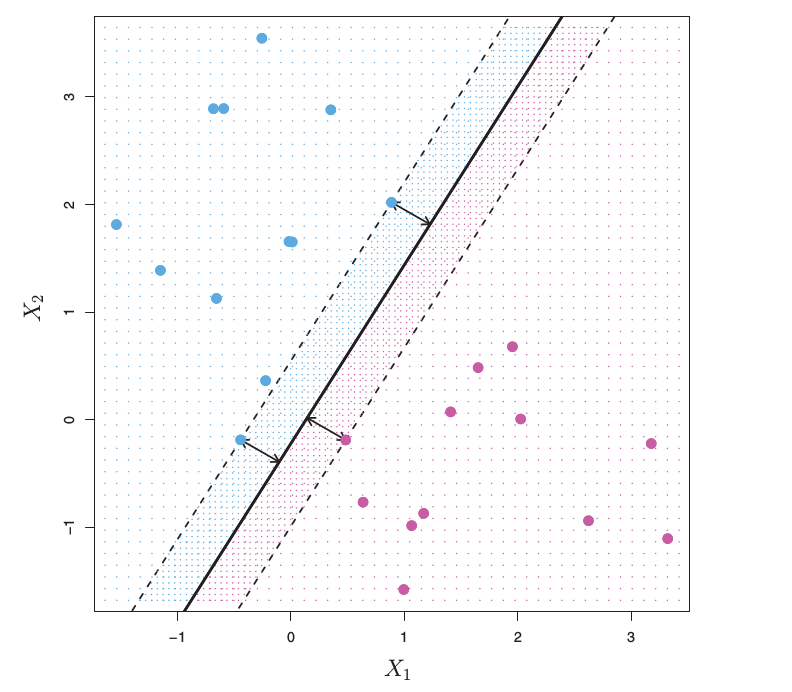
\includegraphics[width=0.5\textwidth]{./Figures/maxim_margin_example.png}
   \caption{Ví dụ về siêu mặt phẳng lề cực đại trong không gian 2 chiều.}
   \label{fig:maxim_margin_example}
\end{figure}

Siêu mặt phẳng được ước lượng bằng cách giải phương trình:


 $$
\large
\begin{cases}
\max\limits_{\beta_0, \beta_1,...,\beta_p}M\\

\sum_{j = 1}^p \beta_j^2 = 1\\

y_i(\beta_0 + \beta_1x_{i2} + ... + \beta_px_{ip}) \geq M \qquad \forall i = 1, 2, ...n
\end{cases}
$$

trong đó $M$ là độ rộng của lề, chúng ta tìm giá trị tối đa cho giá trị này, dưới ràng buộc rằng 
 $$
\large
y_i(\beta_0 + \beta_1x_{i2} + ... + \beta_px_{ip}) \geq M \qquad \forall i = 1, 2, ...n
$$
để đảm bảo rằng mỗi quan sát đều nằm trên đúng phía của siêu mặt phẳng phân loại, với điều kiện rằng $M$ không âm.
Khoảng cách từ quan sát thứ $i$ đến siêu mặt phẳng có thể được tính bằng: 

$$
y_i(\beta_0 + \beta_1x_{i2} + ... + \beta_px_{ip})
$$


\paragraph{Mô hình phân loại véc tơ hỗ trợ}

Mô hình phân loại lề cực đại không thể thực hiện được trong trường hợp không tồn tại một siêu mặt phẳng nào có thể chia tách bộ số liệu ra thành 2 nhóm.

Một cải tiến của mô hình này là mô hình hỗ trợ máy, trong đó siêu mặt phẳng được ước lượng bằng phương trình:

$$
\large
\begin{cases}
\max\limits_{\beta_0, \beta_1,...,\beta_p, \epsilon_1, ... , \epsilon_n}M\\

\sum_{j = 1}^p \beta_j^2 = 1\\

y_i(\beta_0 + \beta_1x_{i2} + ... + \beta_px_{ip}) \geq M(1-\epsilon_i) \\

\epsilon_i \geq 0, \quad \sum_{i = 1}^n \epsilon_i \leq C
\end{cases}
$$

Trong đó $C$ là một tham số không âm do ta lựa chọn. $\epsilon_i$ là các hệ số không âm cho phép quan sát thứ $i$ vi phạm quy tắc của siêu mặt phẳng biên cực đại, với $C$ là giới hạn cho số sai phạm này. Nếu $0 < \epsilon_i < 1$, điểm $i$ nằm ở phía trong biên nhưng vẫn đúng phía của siêu mặt phẳng phân loại. Nếu $\epsilon_i = 1$, điểm $i$ nằm ở sai phía của siêu mặt phẳng phân loại.

\paragraph{Các kernel và mô hình véc tơ hỗ trợ máy}

Mô hình véc tơ hỗ trợ máy (Support Vector Machine) là một mở rộng của mô hình phân loại vectơ hỗ trợ, giúp xây dựng các mô hình phân loại phi tuyến. Mô hình này sử dụng một phép chiếu $\Phi$, chiếu các quan sát từ một không gian không phân biệt tuyến tính lên một chiều không gian mới mà ở đó các quan sát trở nên phân biệt tuyến tính.

Trong thực tế, việc thực hiện phép chiếu $\Phi$ này có thể trở nên rất khó khăn khi kích cỡ của bộ số liệu lớn. \textcite{scholkopf1999advances} chỉ ra rằng đối với một số phép chiếu, để ước lượng được mô hình véc tơ hỗ trợ, chúng ta chỉ cần tính được tích vô hướng của các quan sát trong bộ dữ liệu, thủ thuật này được gọi là thủ thuật kernel. Mô hình véc tơ hỗ trợ sử dụng thủ thuật kernel này được gọi là mô hình véc tơ hỗ trợ máy (SVM). Một cách tổng quát, mô hình SVM ước lượng:

$$
f(x) = \beta_0 + \sum\alpha_i K(x, x_i)
$$

trong đó $\beta0$, $\alpha_i$ là các hệ số cần ước lượng, $K(x, x_i)$ được gọi là hàm kernel, $x_i$ và $x$ lần lượt là véc tơ của quan sát thứ $i$ trong bộ số liệu và vectơ của quan sát mới cần phân loại.

Một số hàm kernel phổ biến được sử dụng rộng rãi là:

\begin{itemize}
  \item{$K(x, x_i) = x_i^T x$}: Hàm kernel tuyến tính, đây thực chất là hàm kernel của mô hình phân loại vec tơ hỗ trợ bình thường.
  \item{$K(x, x_i) =  (1 + \sum_{j = 1}^p x_i x)^d$}: Hàm kernel đa thức với tham số $d$ là bậc của đa thức ước lượng.
  \item{$K(x, x_i) = e^{-\frac{{\|x - x_i\|}^2}{2 \sigma^2}}$}: Hàm kernel tròn với tham số $\sigma$ quyết định bán kính của đường tròn phân chia các quan sát
\end{itemize}

\begin{figure}
  \centering
    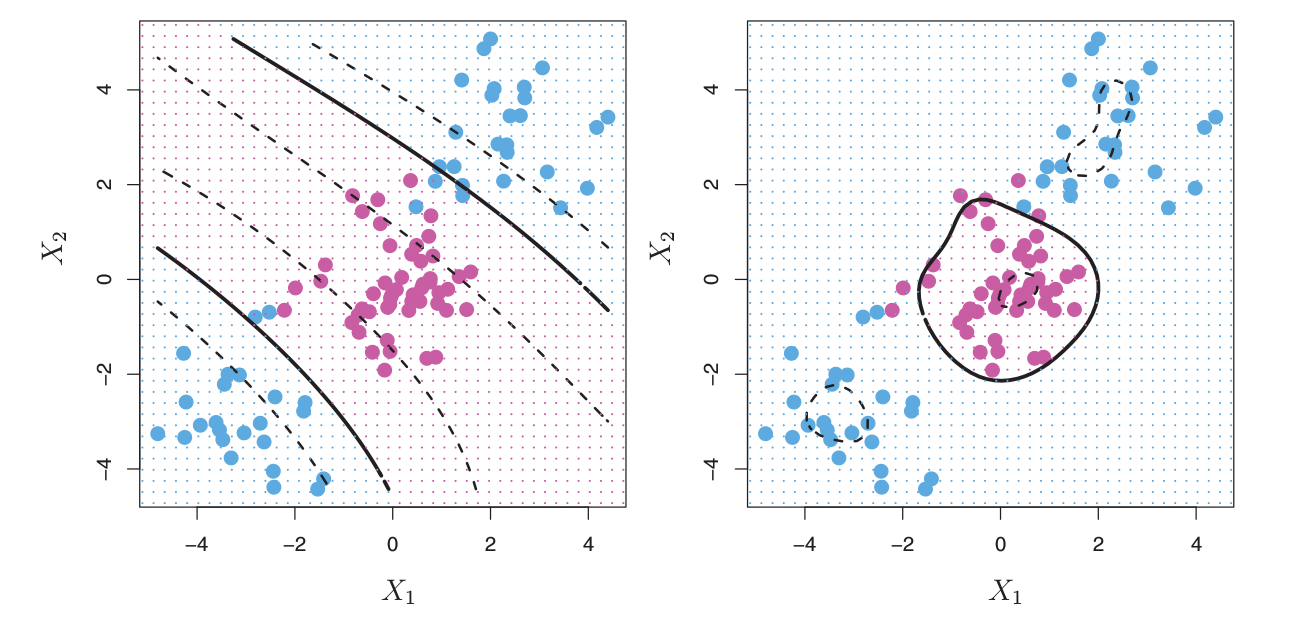
\includegraphics[width=\textwidth]{./Figures/svm_kernel_example.png}
  \caption[Ví dụ về phân loại sử dụng mô hình SVM]{Ví dụ về phân loại sử dụng mô hình SVM sử dụng kernel đa thức với d = 3 (trái) và kernel tròn (phải)}
  \label{fig:svm_kernel_example}
\end{figure}

\subsubsection{Quy trình xây dựng một mô hình véc tơ máy hỗ trợ}

Trong xây dựng một mô hình SVM, việc lựa chọn kernel thích hợp và việc điều chỉnh để có được tham số thích hợp cho kernel đó là yếu tố vô cùng quan trọng. 
\textcite{hsu2003practical} đưa ra một quy trình để có thể đạt được kết quả chấp nhận được đối với hầu hết các trường hợp. Quy trình đó như sau:

\begin{itemize}
  \item Thực hiện chuẩn hoá bộ số liệu
  \item Ưu tiên sử dụng kernel tròn (RBF): $K(x, x_i) = e^{-\frac{{\|x - x_i\|}^2}{2 \sigma^2}}$
  \item Sử dụng kiểm định chéo để tìm tham số tốt nhất cho $C$ và $\sigma$.
  \item Sử dụng tham số $C$ và $\sigma$ tốt nhất ước lượng được để ước lượng trên toàn bộ bộ số liệu dùng để xây dựng mô hình.
  \item Kiểm tra hiệu quả mô hình.
\end{itemize}

Trong bài này ta sẽ đi theo quy trình này để xây dựng mô hình SVM, sử dụng phần mềm \texttt{LIBSVM} \textcite{CC01a}, một phần mềm phổ biến được sử dụng rộng rãi để xây dựng các mô hình SVM.
% \section{Đánh giá mô hình}
% \subsection{Đường ROC và phần diện tích dưới đường cong (AUC)}
% \subsection{Thang đo H}

%%%%%%%%%%%%
% Chương 3 %
%%%%%%%%%%%%

\chapter{Tình huống nghiên cứu}

\section{Số liệu và các biến số}

Chúng ta thực hành trên bộ số liệu mẫu bao gồm 30000 quan sát và 25 biến bao gồm tình trạng trả nợ, các thông tin nhân khẩu học cơ bản cùng với số liệu về tín dụng và tình trạng hồ sơ của các khách hàng thẻ tín dụng ở Đài Loan từ tháng 4 năm 2005 đến tháng 9 năm 2005.

Các tên biến đã được thay đổi để tiện lợi cho việc đọc hiểu và phân tích, cụ thể như sau:

\begin{description}
  \item [\texttt{ID}] Số ID của mỗi khách hàng tín dụng
  \item [\texttt{LIMIT\_BAL}] Lượng tín dụng cho vay tính bằng Đô la Đài Loan (bao gồm cả các khoản vay cá nhân và các khoản vay với thẻ tín dụng phụ)
  \item [\texttt{SEX}] Giới tính (0=Nữ, 1=Nam)
  \item [\texttt{EDUCATION}] (1=sau đại học, 2=đại học, 3=phổ thông, 4=khác)
  \item [\texttt{MARRIAGE}] Trạng thái hôn nhân (1=đã cưới, 2=độc thân, 3=khác)
  \item [\texttt{AGE}] Số tuổi tính bằng năm
  \item [\texttt{PAY\_0}] Tình trạng hồ sơ vào thời điểm tháng 9/2005 (-1=trả đúng hạn, 1=chậm 1 tháng, 2=chậm 2 tháng, ... 8=chậm 8 tháng, 9=chậm 9 tháng hoặc nhiều hơn)
  \item [\texttt{PAY\_2}] Tình trạng hồ sơ vào thời điểm tháng 8/2005 (thang điểm như trên)
  \item [\texttt{PAY\_3}] Tình trạng hồ sơ vào thời điểm tháng 7/2005 (thang điểm như trên)
  \item [\texttt{PAY\_4}] Tình trạng hồ sơ vào thời điểm tháng 6/2005 (thang điểm như trên)
  \item [\texttt{PAY\_5}] Tình trạng hồ sơ vào thời điểm tháng 5/2005 (thang điểm như trên)
  \item [\texttt{PAY\_6}] Tình trạng hồ sơ vào thời điểm tháng 4/2005 (thang điểm như trên)
  \item [\texttt{BILL\_AMT1}] Hóa đơn thanh toán vào thời điểm 9/2005 (Đô la Đài Loan)
  \item [\texttt{BILL\_AMT2}] Hóa đơn thanh toán vào thời điểm 8/2005 (Đô la Đài Loan)
  \item [\texttt{BILL\_AMT3}] Hóa đơn thanh toán vào thời điểm 7/2005 (Đô la Đài Loan)
  \item [\texttt{BILL\_AMT4}] Hóa đơn thanh toán vào thời điểm 6/2005 (Đô la Đài Loan)
  \item [\texttt{BILL\_AMT5}] Hóa đơn thanh toán vào thời điểm 5/2005 (Đô la Đài Loan)
  \item [\texttt{BILL\_AMT6}] Hóa đơn thanh toán vào thời điểm 4/2005 (Đô la Đài Loan)
  \item [\texttt{PAY\_AMT1}] Lượng tiền đã thanh toán vào thời điểm tháng 9/2015 (Đô la Đài Loan)
  \item [\texttt{PAY\_AMT2}] Lượng tiền đã thanh toán vào thời điểm tháng 8/2015 (Đô la Đài Loan)
  \item [\texttt{PAY\_AMT3}] Lượng tiền đã thanh toán vào thời điểm tháng 7/2015 (Đô la Đài Loan)
  \item [\texttt{PAY\_AMT4}] Lượng tiền đã thanh toán vào thời điểm tháng 6/2015 (Đô la Đài Loan)
  \item [\texttt{PAY\_AMT5}] Lượng tiền đã thanh toán vào thời điểm tháng 5/2015 (Đô la Đài Loan)
  \item [\texttt{PAY\_AMT6}] Lượng tiền đã thanh toán vào thời điểm tháng 4/2015 (Đô la Đài Loan)
  \item [\texttt{DEFAULT}] Có trả nợ hay không (1=có, 0=không)
\end{description}


Hình \ref{fig:corr_mat} (trang \pageref{fig:corr_mat}) mô tả ma trận hệ số tương quan Pearson giữa các biến số trong bộ số liệu. 
Lưu ý tương quan giữa các biến trong nhóm biến \texttt{PAY} (tình trạng hồ sơ) và 
giữa các biến trong nhóm biến \texttt{BILL\_AMT} (hoá đơn thanh toán) là khá cao, thể hiện sự tương đồng cao về mặt thông tin thể hiện của các biến này.
Trong số các biến trong bộ số liệu, các biến \texttt{PAY} là có thể hiện tương quan dương với biến \texttt{DEFAULT}, gợi ý rằng chúng ta có thể sử dụng biến này là biến chính để dự đoán tỉ lệ vỡ nợ của khách hàng.

\begin{figure}[h]
\centering
\capstart
\begin{knitrout}\small
\definecolor{shadecolor}{rgb}{0.969, 0.969, 0.969}\color{fgcolor}
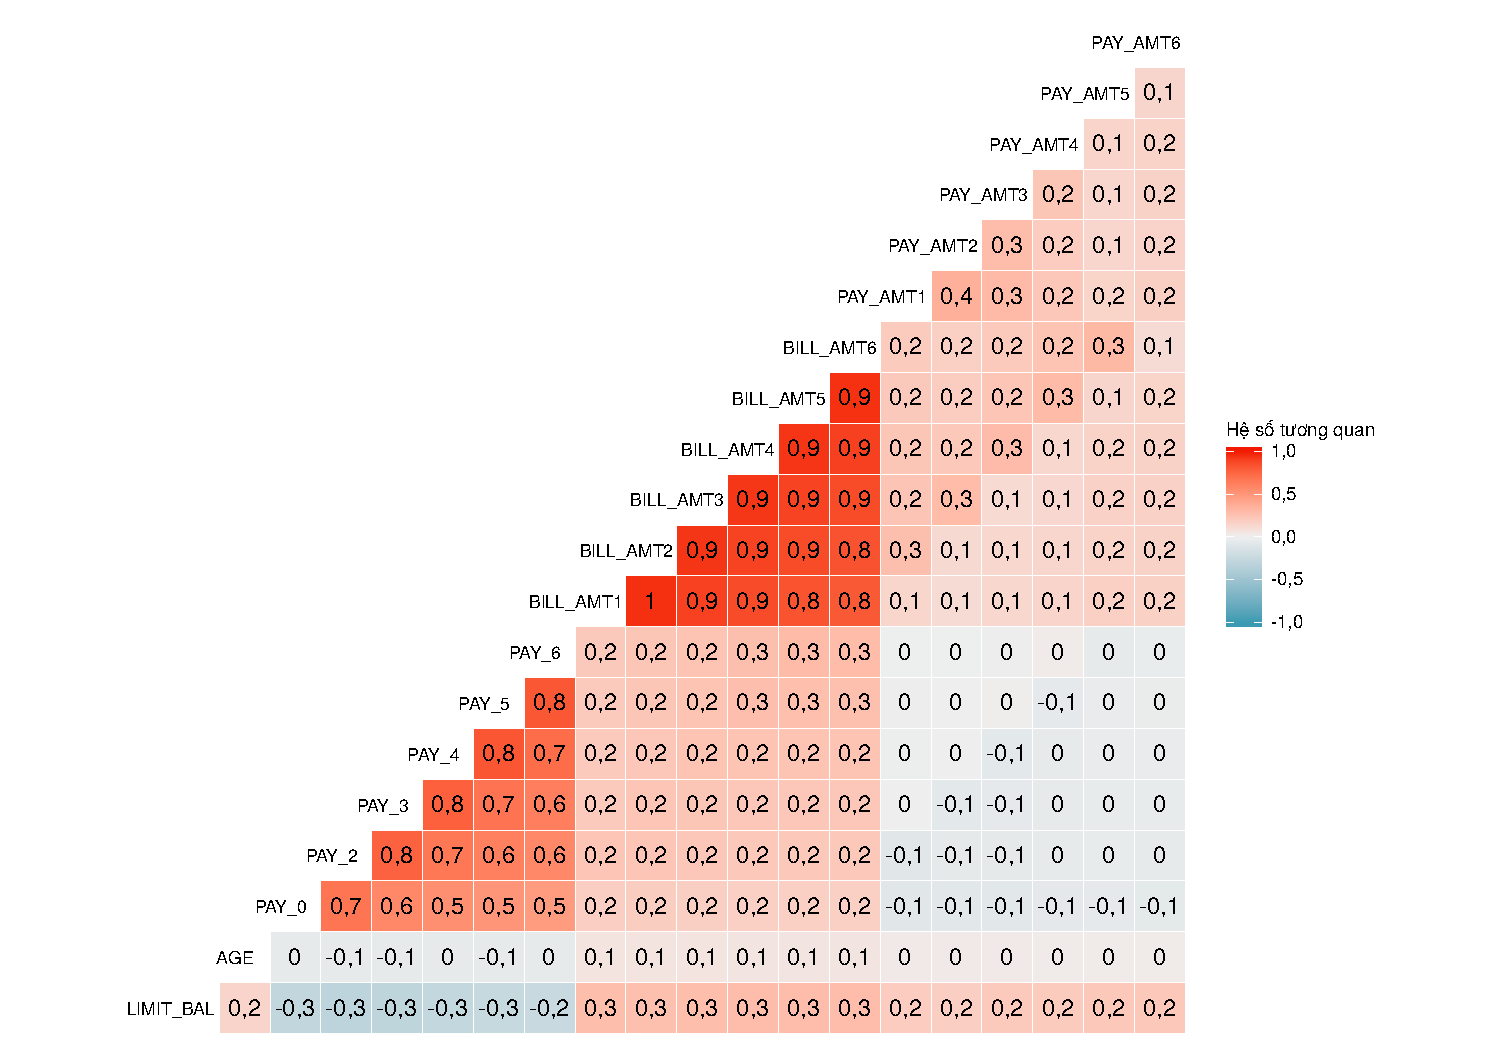
\includegraphics[width=\textwidth]{Figures/corr_mat-1} 

\end{knitrout}
\caption[Ma trận hệ số tương quan Pearson]{Ma trận hệ số tương quan Pearson giữa các biến trong bộ số liệu.}
\label{fig:corr_mat}
\end{figure}

Để có cái nhìn cụ thể hơn vào bộ số liệu này, chúng ta sử dụng phương pháp phân tích thành phần chính (PCA - Principal Component Analysis) để phân tích bộ số liệu.
Với phương pháp này, chúng ta tìm một hệ tọa độ trực giao mới để thể hiện bộ số liệu, sao cho với thành phần chính thứ nhất (chiều thứ nhất của hệ tọa độ mới) thể hiện được nhiều nhất có thể thông tin của bộ số liệu, thành phần chính thứ hai (chiều thứ hai của hệ tọa độ mới) thể hiện nhiều nhất có thể lượng thông tin còn lại của bộ số liệu, v...v... Lưu ý rằng vì các biến trong bộ số liệu có thang đo khác nhau, để đảm bảo hiệu quả cho phương pháp phân tích đa biến này, chúng ta chuẩn hóa các biến trước khi thực hiện PCA. Đồng thời, các biến phân loại như \texttt{EDUCATION} và \texttt{MARRIAGE} cũng được lược bỏ.

\begin{figure}[h]
\centering
\capstart
\begin{knitrout}\small
\definecolor{shadecolor}{rgb}{0.969, 0.969, 0.969}\color{fgcolor}
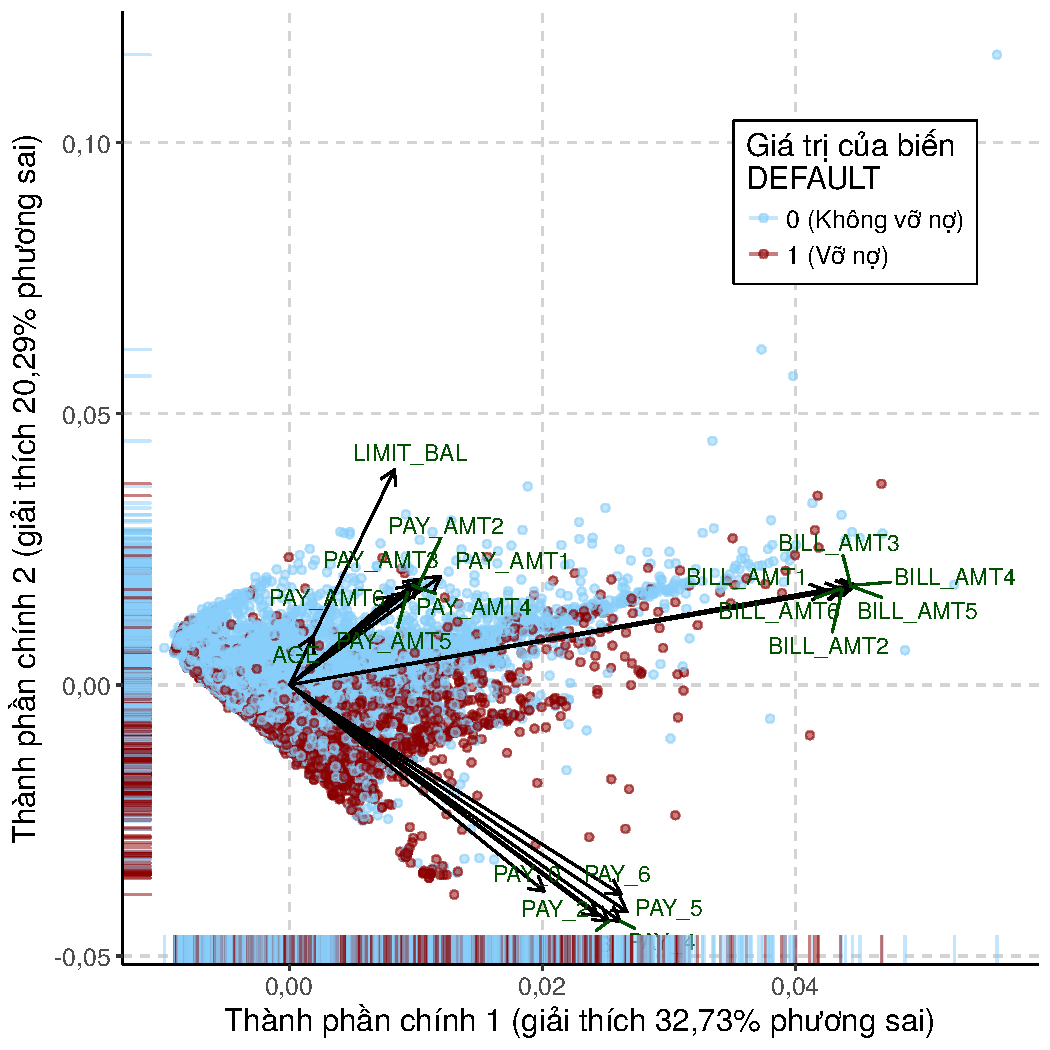
\includegraphics[width=10cm,height=10cm]{Figures/pca-1} 

\end{knitrout}
\caption{Phép chiếu bộ số liệu trên hai thành phần chính.}
\label{fig:pca}
\end{figure}

Phép chiếu của các biến và các quan sát trong bộ số liệu trên hai thành phần chính đầu tiên được thể hiện trong hình \ref{fig:pca} (trang \pageref{fig:pca}), với mỗi véc tơ thể hiện một biến và mỗi điểm thể hiện một quan sát trong bộ số liệu. Các quan sát thuộc vào nhóm vỡ nợ (biến \texttt{DEFAULT} bằng 1) có màu đỏ và các quan sát thuộc nhóm không vỡ nợ (biến \texttt{DEFAULT} bằng 0) có màu xanh. 
Quan sát đồ thị này, chúng ta nhận thấy các quan sát thuộc nhóm vỡ nợ (màu đỏ) tập trung nhiều ở phía dưới đồ thị, hay là giá trị của các biến này chiếu trên thành phần chính thứ 2 (trục tung) là thấp hơn. 
Như chúng ta nhận xét ở ma trận hệ số tương quan phía trên, véc tơ chiếu các biến thuộc cùng nhóm \texttt{PAY}, \texttt{PAY\_ATM} và \texttt{BILL\_ATM} nằm khá gần nhau, thể hiện mức độ tương quan cao giữa các biến số thuộc cùng một trong ba nhóm này. Các biến thuộc nhóm \texttt{PAY} có hướng trùng với hướng phân bố của các quan sát thuộc nhóm vỡ nợ, trong khi các biến thuộc nhóm \texttt{PAY\_ATM} có hướng trùng với hướng phân bố của các quan sát thuộc nhóm không vỡ nợ, gợi ý tiềm năng dùng để dự báo của các nhóm biến này. 
Ngoài ra các quan sát nhóm vỡ nợ cũng có xu hướng thể hiện cao trên biến 
\texttt{SEX}. Nhóm các quan sát không vỡ nợ cũng phân bố nhiều theo chiều tăng của các biến \texttt{AGE} và \texttt{LIMIT\_BAL}.

Lưu ý rằng đồ thị \ref{fig:pca} chỉ thể hiện $\text{55,7}$ phần trăm lượng thông tin của bộ số liệu, chưa kể các biến phân loại như \texttt{EDUCATION} hay \texttt{MARRIAGE}. Bằng cách sử dụng các phương pháp phân tích cụ thể hơn, chúng ta có thể đưa ra một mô hình phân loại chính xác hơn đối với khả năng vỡ nợ của các khách hàng dùng thẻ tín dụng trong bộ số liệu này.

Trong 30000 quan sát của bộ số liệu này, sau khi làm sạch, chúng ta chọn ngẫu nhiên 75\% (Khoảng hơn 22000 quan sát) để xây dựng các mô hình. Số lượng quan sát còn lại sẽ được dùng để kiểm tra các mô hình xây dựng được và cho chúng ta cái nhìn về hiệu quả của chúng.


\section{Xây dựng mô hình logit}

\subsection{Tiền xử lý bộ số liệu}
Mô hình logit giả định xác suất dự báo  $P(y = 1|X)$  phân phối chuẩn với trung bình là 0,5 và thực hiện ước lượng có hiệu quả hơn trên bộ số liệu có tỉ lệ biến phụ thiộc là 0,5. 
Tuy nhiên trong bộ số liệu chúng ta nghiên cứu này, tỷ lệ  $\texttt{DEFAULT} = 1$ là $22.34\%$.
Để đảm bảo cho hiệu quả của mô hình logit, trong bộ số liệu dùng để ước lượng mô hình, chúng ta lấy tập con của số mẫu thuộc nhóm $\texttt{DEFAULT} = 1$ một cách ngẫu nhiên, sao cho tỷ lệ  $P(\texttt{DEFAULT} = 1)$ trong bộ số liệu ước lượng bây giờ là 0,5. 

\subsection{Ước lượng mô hình} 


Chúng ta thực hiện mô hình logit, sử dụng phương pháp Lasso để giới hạn giá trị của các hệ số ước lượng. 
Với mỗi gía trị của tham số $\lambda$, giá trị của các hệ số ước lượng $\beta$ càng bị ràng buộc chặt, các hệ số ước lượng có giá trị bằng 0 có thể coi là bị loại khỏi mô hình.

\begin{figure}[h]
\centering
\capstart
\begin{knitrout}\small
\definecolor{shadecolor}{rgb}{0.969, 0.969, 0.969}\color{fgcolor}
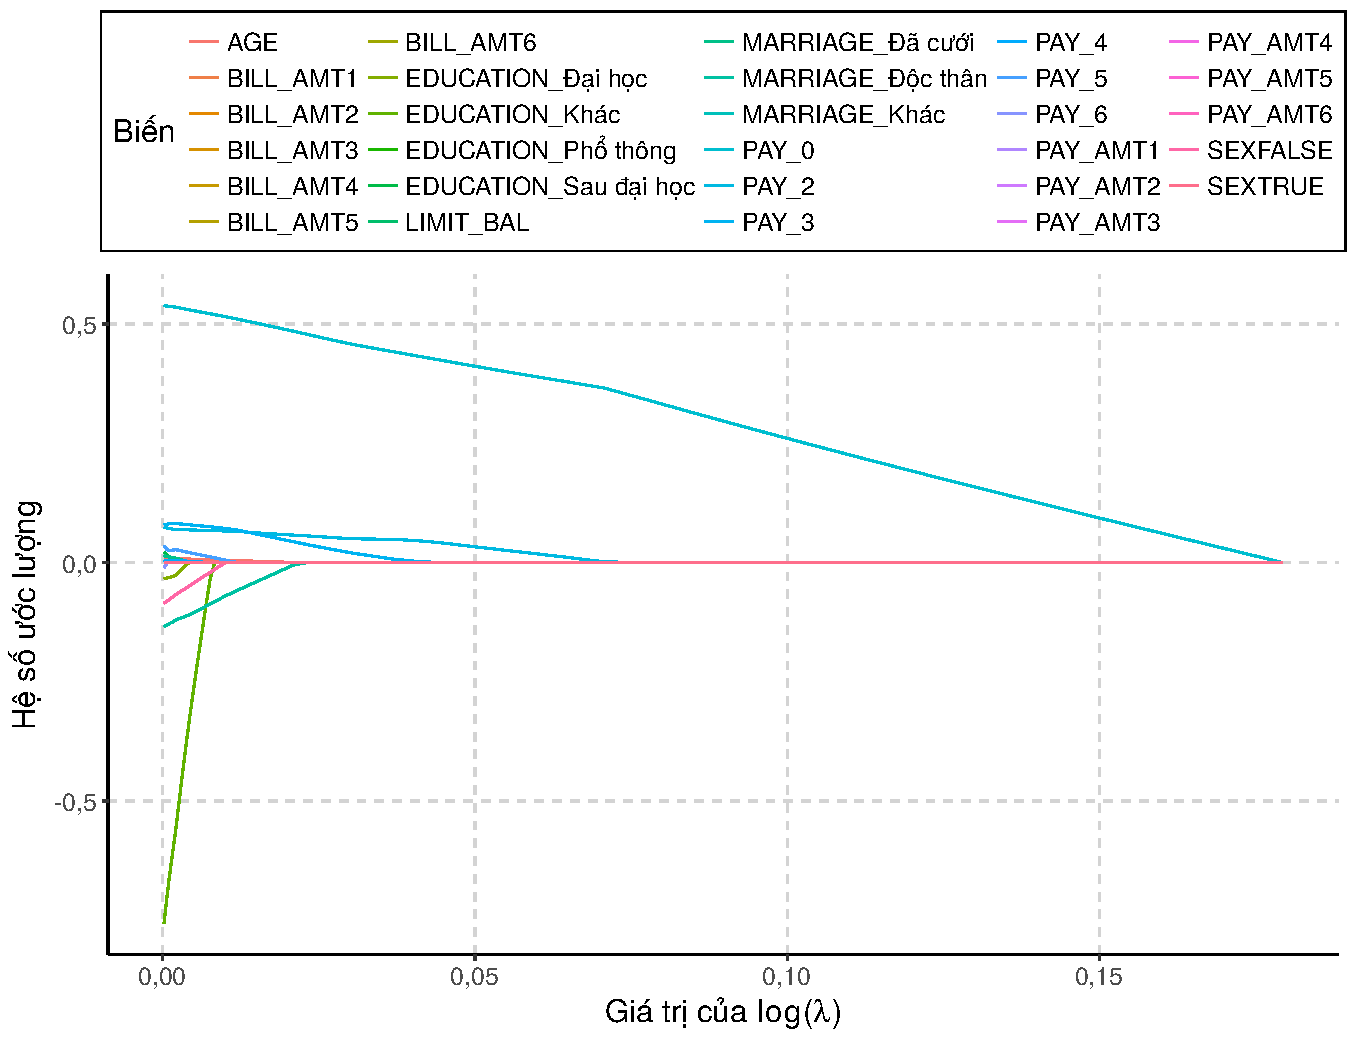
\includegraphics[width=\textwidth,height=12cm]{Figures/lasso_coef-1} 

\end{knitrout}
\caption{Giá trị ước lượng của các hệ số theo chiều tăng của $\log(\lambda)$}
\label{fig:lasso_coef}
\end{figure}

Hình \ref{fig:lasso_coef} mô tả xu hướng của các hệ số ước lượng $\beta$ khi giá trị của $\log\lambda$ thay đổi.
Với hướng tăng của $\log\lambda$ các biến thuộc nhóm \texttt{BILL} nhanh chóng hội tụ về $0$, thể hiện mức ý nghĩa thống kê thấp của các hệ số này trong mô hình. Trong khi đó, các biến thuộc nhóm \texttt{PAY} chậm hội tụ về $0$ hơn, với biến \texttt{PAY\_0} là biến cuối cùng có hệ số ước lượng $\beta$ tương ứng hội tụ về 0.
Với các giá trị $\lambda$ lớn hơn từ sau thời điểm này, có thể nói mô hình chỉ còn hệ số chặn $\beta_0$.

Để xác định giá trị hợp lý cho tham số $\lambda$ trong mô hình này. Chúng ta thực hiện bằng cách chia bộ số liệu thử nghiệm thành 10 phần nhỏ, chạy mô hình logit sử dụng phương pháp Lasso này trên từng bộ số liệu con này, rồi kiểm định kết quả mô hình dựa trên các bộ số liệu còn lại.
Từ kết quả của 10 phép ước lượng kiểm định chéo này, chúng ta có thể tính được giá trị trung bình của Deviance tại các giá trị của $\lambda$, qua đó chúng ta có thể xác định được giá trị của $\lambda$ mà Deviance là thấp nhất.

\begin{figure}
\centering
\capstart
\begin{knitrout}\small
\definecolor{shadecolor}{rgb}{0.969, 0.969, 0.969}\color{fgcolor}
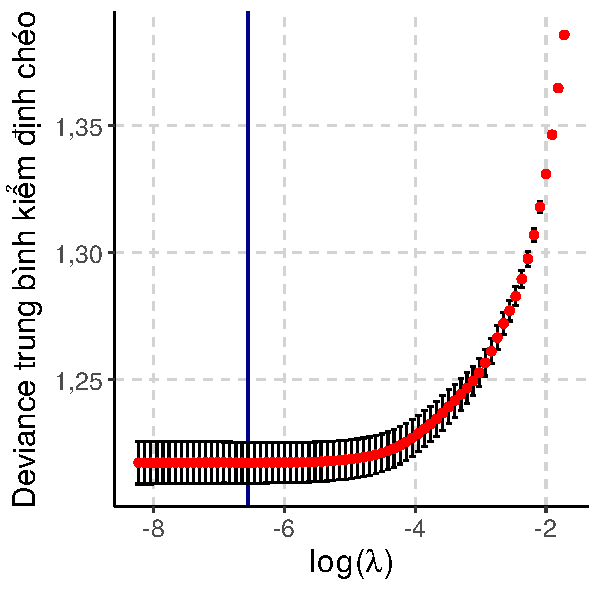
\includegraphics[width=10cm,height=10cm]{Figures/lasso_cv-1} 

\end{knitrout}
\caption{Giá trị trung bình của Deviance tương ứng với mỗi giá trị tương ứng của $\lambda$}
\label{fig:lasso_cv}
\end{figure}

Hình \ref{fig:lasso_cv} mô tả mối quan hệ của Deviance (trên trục tung) khi giá trị của $\lambda$ thay đổi (giá trị của $\lambda$ trên trục hoành đã được logarit hóa). Các chấm màu đỏ biểu diễn giá trị Deviance trung bình của kiểm định chéo tại các giá trị khác nhau của $\log(\lambda)$, thanh màu đen thể hiện sai số chuẩn tương ứng của giá trị trung bình này. Đường kẻ dọc màu xanh đậm đánh dấu giá trị của $\log(\lambda)$ mà tại đó gía trị của Deviance là thấp nhất($\lambda \approx\ $\text{0,002725}), tương đương với giá trị của $\lambda$ mà chúng ta lựa chọn cho mô hình này.

Hệ số ước lượng $\beta$ của mô hình được thể hiện trong bảng \ref{tab:lasso_final}). 

% latex table generated in R 3.4.0 by xtable 1.8-2 package
% Sat May 27 03:05:18 2017
\begin{table}[htb!]
\centering
\begin{tabular}{ll}
  \hline
Tên biến & Hệ số \\ 
  \hline
Hệ số chặn & -0,0790705 \\ 
  LIMIT\_BAL & -0,0949844 \\ 
  SEXFALSE & -0,0617021 \\ 
  SEXTRUE & 0,0002595 \\ 
  EDUCATION\_Đại học & -0,01836 \\ 
  EDUCATION\_Khác & -0,4910211 \\ 
  MARRIAGE\_Đã cưới & 0,0068734 \\ 
  MARRIAGE\_Độc thân & -0,1172755 \\ 
  AGE & 0,0725433 \\ 
  PAY\_0 & 0,6006201 \\ 
  PAY\_2 & 0,0829978 \\ 
  PAY\_3 & 0,0974986 \\ 
  PAY\_4 & 0,0049178 \\ 
  PAY\_5 & 0,0288028 \\ 
  BILL\_AMT1 & -0,1086513 \\ 
  PAY\_AMT1 & -0,2221284 \\ 
  PAY\_AMT2 & -0,1073109 \\ 
  PAY\_AMT3 & -0,0552885 \\ 
  PAY\_AMT4 & -0,0642869 \\ 
  PAY\_AMT5 & -0,0166451 \\ 
  PAY\_AMT6 & -0,0578704 \\ 
   \hline
\end{tabular}
\caption{Hệ số ước lượng} 
\label{tab:lasso_final}
\end{table}



\section{Xây dựng mô hình SVM}

\subsection{Tiền xử lý bộ số liệu}
Trong số liệu được sử dụng để xây dựng mô hình SVM cũng được xử lý tương tự như xử lý cho mô hình Logit.

\subsection{Xây dựng mô hình SVM}
% Sig range.... from 0.1 - 0.9 quantile
Theo \textcite{963105}, tham số $\sigma$ hiệu qủa cho mô hình SVM đều nằm trong khoảng phân vị 0.1 đến phân vị 0.9 của $\|x - x_i\|$. Các giá trị phân vị của $\|x - x_i\|$ trong bộ số liệu đã được xử lý như sau:

\begin{knitrout}\small
\definecolor{shadecolor}{rgb}{0.969, 0.969, 0.969}\color{fgcolor}\begin{kframe}
\begin{verbatim}
##         90%         50%         10% 
## 0,009507368 0,027192205 0,059278172
\end{verbatim}
\end{kframe}
\end{knitrout}



Để lựa chọn tham số hợp lý cho $C$ và $\sigma$ chúng ta thực hiện phép thử với từng cặp của hai tham số này. Với mỗi cặp của $C$ và $\sigma$, chúng ta thực hiện phép kiểm định chéo 5 lớp trên bộ số liệu dùng để xây dựng mô hình và tính phần diện tích dưới đường cong ROC trung bình.

\begin{figure}[h]
\centering
\capstart
\begin{knitrout}\small
\definecolor{shadecolor}{rgb}{0.969, 0.969, 0.969}\color{fgcolor}
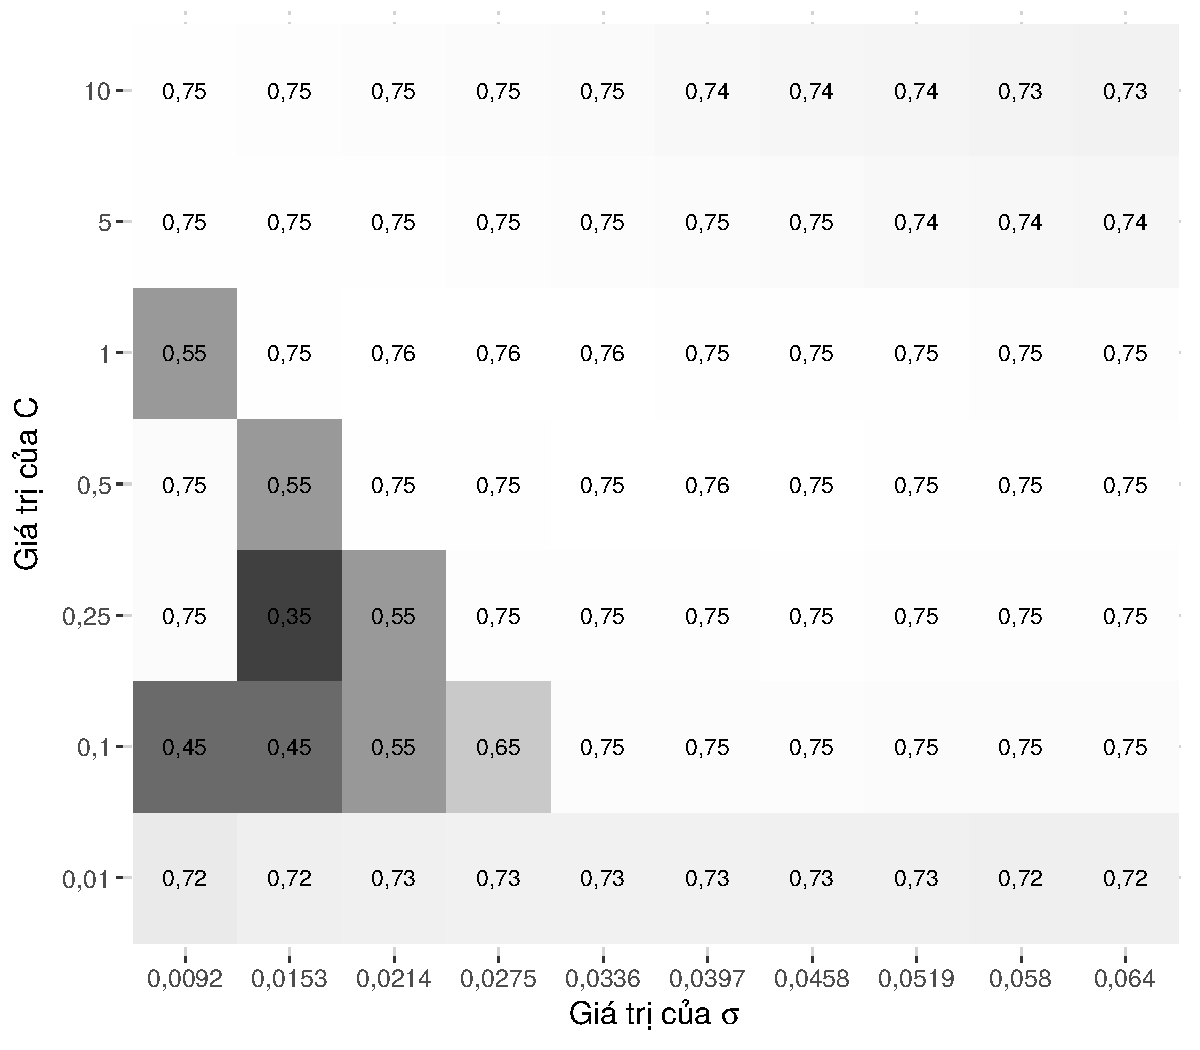
\includegraphics[width=\textwidth]{Figures/svm_train-1} 

\end{knitrout}
\caption{Kết quả SVM cho các giá trị khác nhau cuả tham số $C$ và $\sigma$}
\label{fig:svm_train}
\end{figure}

Hình \ref{fig:svm_train} cho thấy kết quả của phép thử này.  Giá trị lớn nhất của chỉ số ROC đạt được tại $C = 1$ và $\sigma \approx 0.0275$, sử dụng giá trị tham số này, ta ước lượng mô hình SVM trên toàn bộ tập số liệu dùng để xây dựng mô hình:

\begin{knitrout}\small
\definecolor{shadecolor}{rgb}{0.969, 0.969, 0.969}\color{fgcolor}\begin{kframe}
\begin{verbatim}
## Support Vector Machine object of class "ksvm" 
## 
## SV type: C-svc  (classification) 
##  parameter : cost C = 1 
## 
## Gaussian Radial Basis kernel function. 
##  Hyperparameter : sigma =  0,0336744006003365 
## 
## Number of Support Vectors : 6709 
## 
## Objective Function Value : -6079,479 
## Training error : 0,276116
\end{verbatim}
\end{kframe}
\end{knitrout}



\section{Kết luận về kết quả ước lượng của các mô hình}

\subsection{Nhận xét về hiệu quả của các mô hình}

\subsubsection{Nhận xét mô hình Logit}

%% \begin{figure}
%% \centering
%% \capstart

%% <<lasso_confusion_mat, fig.width=5,fig.height=4,out.width='10cm', out.heith='8cm'>>=
%% result <- data_frame(
%%   Predict = (predict.glmnet(lasso_fit, newx = test_x_set,
%%                            s = lasso_cv$lambda.min)[,1] > 0.5),
%%   Actual = test_set$DEFAULT
%% ) %>% table() %>% as.data.frame(stringsAsFactors = FALSE) %>%
%%   mutate(color = ifelse(Predict == Actual, Freq, -1*Freq),
%%          percent = round(Freq/sum(Freq) * 100, 2))
%% result[result == TRUE] <- "Vỡ nợ"
%% result[result == FALSE] <- "Không vỡ nợ"

%% result %>%  
%%   ggplot(aes(y = Predict, x = Actual)) + 
%%   geom_tile(aes(fill = color), color = "black", size = 1) +
%%   geom_text(aes(label = paste0(Freq,"\n(", percent,"%)"))) +
%%   scale_fill_gradient2(low = "red", high = "light blue") +
%%   labs(x = "Giá trị thực", y = "Giá trị dự báo") +
%%   theme(legend.position = "none", 
%%         panel.grid.major = element_blank(),
%%         axis.line = element_blank(),
%%         axis.ticks = element_blank())
%% @
%% \caption{Confusion matrix cho mô hình Logit (phương pháp Lasso)}
%% \label{fig:lasso_confusion_mat}
%% \end{figure}

%% Chúng ta sử dụng mô hình ước lượng được để dự báo trên tập số liệu kiểm tra. Hình \ref{fig:lasso_confusion_mat} minh họa một ma trận thể hiện độ chính xác của mô hình khi áp dụng lên tập số liệu kiểm tra, với màu xanh thể hiện các quan sát được dự đoán đúng và màu đỏ thể hiện các quan sát được dự đoán sai.

%% Trong tổng cộng nrow(test_set) dòng của bộ số liệu dùng để kiểm tra, có sum(result[result$Actual  == "Vỡ nợ", "Freq"]) trường hợp vỡ nợ, trong đó mô hình dự đoán đúng sum(result[result$Actual == "Vỡ nợ" & result$Predict == "Vỡ nợ", "Freq"]) trường hợp. 
%% Đồng thời, trong các quan sát thuộc nhóm không vỡ nợ còn lại, có sum(result[result$Actual == "Không vỡ nợ" & result$Predict == "Vỡ nợ", "Freq"]) quan sát bị mô hình đánh giá nhầm là có vỡ nợ.

%% Nhìn chung tỉ lệ dự đoán chính xác của mô hình trên tập số liệu kiểm tra là sum(result[result$color > 0, "percent"])\%, tỷ lệ của sai lầm loại I (không vỡ nợ nhưng mô hình dự đoán là có) là sum(result[result$Actual == "Không vỡ nợ" & result$Predict == "Vỡ nợ", "percent"])\%, tỷ lệ của sai lầm loại II (có vỡ nợ nhưng dự đoán là không vỡ nợ) là sum(result[result$Predict == "Không vỡ nợ" & result$Actual == "Vỡ nợ", "percent"])\%.

Tuy là một trong những mô hình được sử dụng rộng rãi trong các bài toán phân loại nhưng về bản chất mô hình Logit lại là một mô hình hồi quy với giá trị hồi quy chúng ta thu được là xác suất vỡ nợ $P(\texttt{DEFAULT} = \texttt{TRUE})$. Với các hệ số của mô hình ước lượng được ở bảng \ref{tab:lasso_final}, chúng ta tính được xác suất $P$ tương ứng của các quan sát trong bộ dữ liệu dùng để kiểm định mô hình. 

\begin{figure}[h]
\centering
\capstart
\begin{knitrout}\small
\definecolor{shadecolor}{rgb}{0.969, 0.969, 0.969}\color{fgcolor}
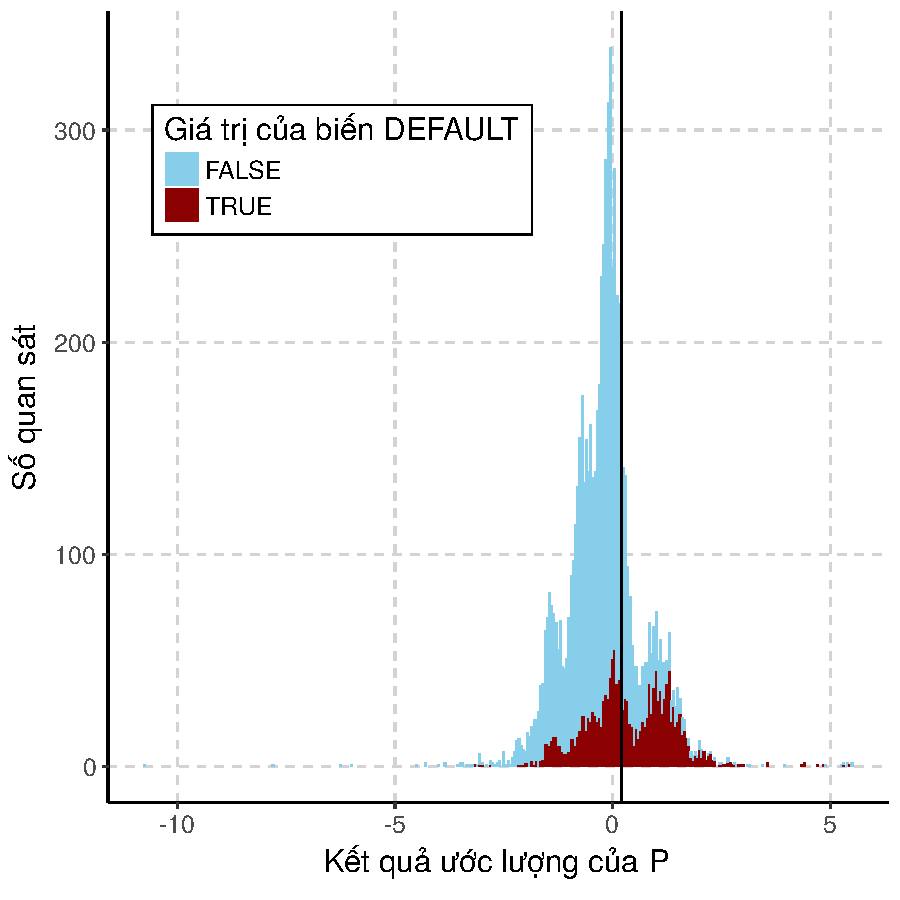
\includegraphics[width=12cm]{Figures/lasso_dist-1} 

\end{knitrout}

\caption{Phân bố giá trị ước lượng được của biến \texttt{DEFAULT}}
\label{fig:lasso_dist}
\end{figure}

Hình \ref{fig:lasso_dist} biểu diễn phân bố của các quan sát trong tập dữ liệu kiểm định đối với giá trị $P$ ước lượng được, với màu đỏ thể hiện cho các quan sát thuộc nhóm vỡ nợ ($\texttt{DEFAULT} = \texttt{TRUE}$) và màu xanh thể hiện cho các quan sát thuộc nhóm không vỡ nợ ($\texttt{DEFAULT} = \texttt{FALSE}$). Chúng ta có thể thấy thang đo $P$ ước lượng được của mô hình chưa thực sự tách các quan sát có giá trị \texttt{DEFAULT} khác nhau ra làm hai phân bố riêng biệt mà vẫn có phần chồng lên nhau giữa phân bố của hai nhóm giá trị. 

Đường thẳng màu đen trong hình thể hiện một điểm cắt cho các quan sát tại giá trị $P = 0,2$. Với mỗi một giá trị khác nhau cho điểm cắt mà ta lựa chọn, chúng ta đánh đổi giữa khả năng dự đoán chính xác cho các điểm thuộc phía bên phải đường cắt (độ nhạy) và khả năng dự báo đúng các điểm nằm phía bên trái đường cắt (độ đặc trưng). Khi giá trị của điểm cắt tăng, độ đặc trưng tăng, độ nhạy giảm và ngược lại.

\begin{figure}[h]
\centering
\capstart
\begin{knitrout}\small
\definecolor{shadecolor}{rgb}{0.969, 0.969, 0.969}\color{fgcolor}
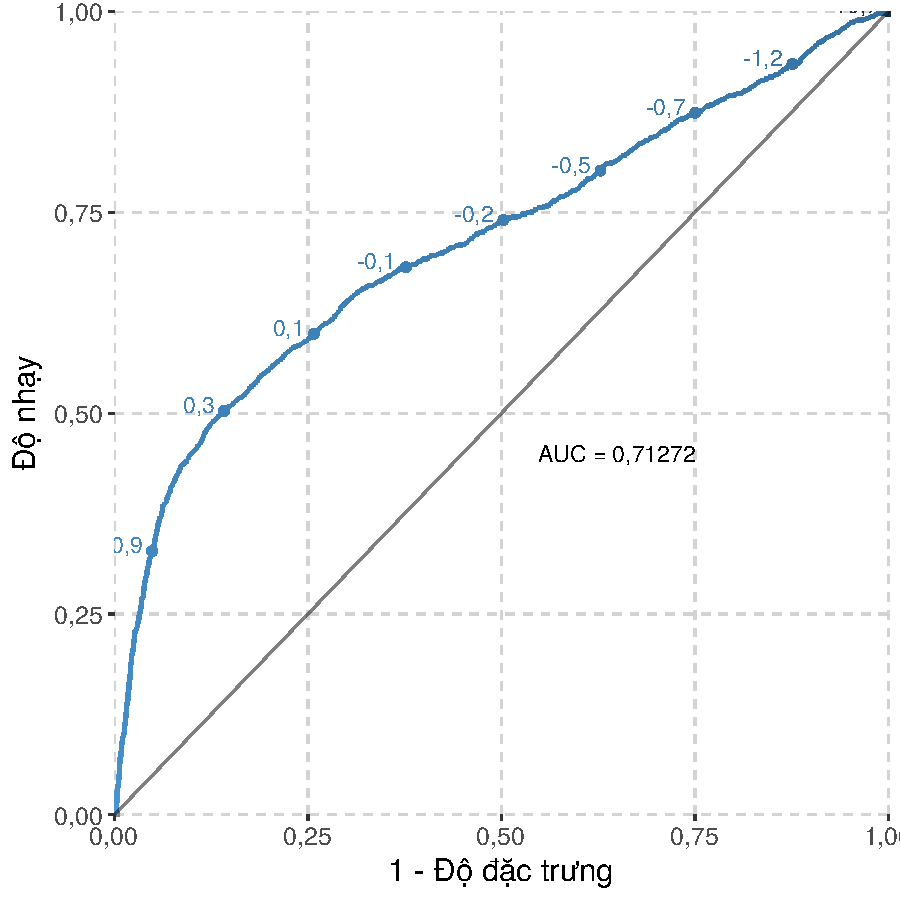
\includegraphics[width=12cm]{Figures/lasso_roc-1} 

\end{knitrout}
\caption{Biểu đồ ROC cho kết quả ước lượng của mô hình Logit}
\label{fig:lasso_roc}
\end{figure}

Sự đánh đổi giữa độ đặc trưng và độ nhạy được biểu diễn bởi đường cong ROC (Hình \ref{fig:lasso_roc}). Một mô hình có khả năng dự báo chính xác càng cao thì phần diện tích dưới đường cong càng lớn. Trong trường hợp này, phần diện tích dưới đường cong là $AUC = \text{0,7127241}$. Ta có thể thấy, với điểm cắt nằm trong khoảng từ $0,1$ đến $0,3$, đường ROC có vẻ cách xa nhất so với đường chéo $45^\circ$, gợi ý rằng điểm cắt tối ưu có thể nằm trong khoảng này.


\subsubsection{Nhận xét mô hình SVM}
Chúng ta sử dụng tiếp tục sử dụng mô hình SVM ước lượng được để dự báo trên tập số liệu kiểm tra. Hình \ref{fig:svm_confution_mat} minh họa một ma trận (confusion matrix) thể hiện độ chính xác của mô hình khi áp dụng lên tập số liệu kiểm tra, với màu xanh thể hiện các quan sát được dự đoán đúng và màu đỏ thể hiện các quan sát bị dự đoán sai.

\begin{figure}[h]
\centering
\capstart

\begin{knitrout}\small
\definecolor{shadecolor}{rgb}{0.969, 0.969, 0.969}\color{fgcolor}
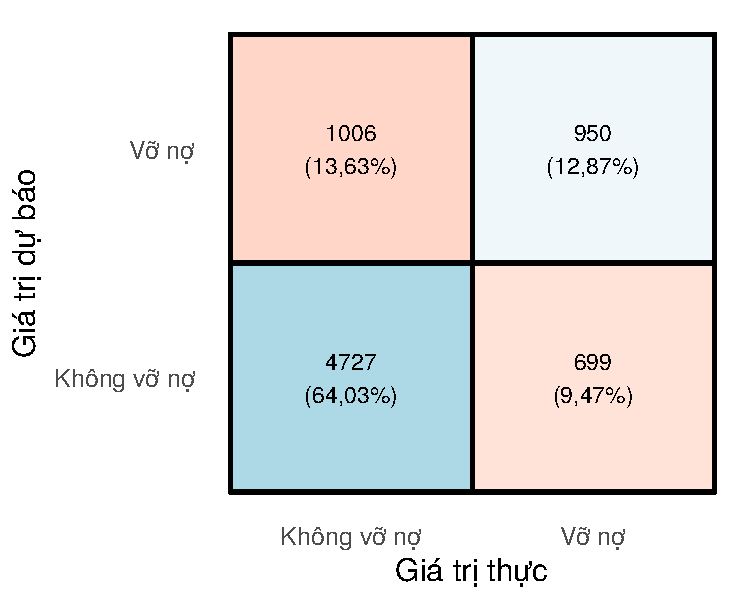
\includegraphics[width=10cm]{Figures/svm_confusion_mat-1} 

\end{knitrout}
  
\caption{Confusion matrix cho mô hình SVM (radial kernel)}
\label{fig:svm_confution_mat}
\end{figure}



Trong tổng cộng \text{7382} dòng của bộ số liệu dùng để kiểm tra, có \text{1649} trường hợp vỡ nợ, trong đó mô hình dự đoán đúng \text{950} trường hợp. Đồng thời, trong các quan sát thuộc nhóm không vỡ nợ còn lại, có \text{1006} quan sát bị mô hình đánh giá nhầm là có vỡ nợ.

% latex table generated in R 3.4.0 by xtable 1.8-2 package
% Sat May 27 03:05:30 2017
\begin{table}[htb!]
\centering
\begin{tabular}{lrlr}
  \hline
  \hline
Accuracy & 0,769033 & Sensitivity & 0,485685 \\ 
  Kappa & 0,375717 & Specificity & 0,871176 \\ 
  AccuracyLower & 0,759246 & Pos Pred Value & 0,576107 \\ 
  AccuracyUpper & 0,778607 & Neg Pred Value & 0,824525 \\ 
  AccuracyNull & 0,735031 & Precision & 0,576107 \\ 
  AccuracyPValue & 0,000000 & Recall & 0,485685 \\ 
  McnemarPValue & 0,000000 & F1 & 0,527046 \\ 
   &  & Prevalence & 0,264969 \\ 
   &  & Detection Rate & 0,128691 \\ 
   &  & Detection Prevalence & 0,223381 \\ 
   &  & Balanced Accuracy & 0,678430 \\ 
   \hline
\end{tabular}
\caption{Một số chỉ tiêu phân tích kết quả phân loại của mô hình SVM} 
\label{tab:svm_cm}
\end{table}


Một số chỉ tiêu của ma trận này được thể hiện ở bảng \ref{tab:svm_cm}. Ta có thể thấy độ nhạy (sensitivity) của mô hình là $\approx 0,48 \%$, độ đặc trưng (specificity) của mô hình là $\approx 0,87 \%$


Nhìn chung tỉ lệ dự đoán chính xác của mô hình trên tập số liệu kiểm tra là \text{0,7690328}\%, tỷ lệ của sai lầm loại I (không vỡ nợ nhưng mô hình dự đoán là có) là \text{13,63}\%, tỷ lệ của sai lầm loại II (có vỡ nợ nhưng dự đoán là không vỡ nợ) là \text{9,47}\%.



\subsubsection{So sánh giữa hai mô hình}

Mô hình Logit cho ta một thang đo $P$ để xếp hạng các quan sát, tuy nhiên mô hình SVM lại chỉ đưa ra một mặt cắt trong không gian để phân loại các quan sát thành hai nhóm. Để có thể so sánh một cách sơ bộ về khả năng phân biệt của hai mô hình, chúng ta lựa chọn một điểm cắt cho mô hình Logit mà tại đó khả năng phân loại khách hàng vỡ nợ của mô hình (sensitivity) tương đồng với của mô hình SVM. Confusion matrix tương ứng của Logit tại điểm cắt này được thể hiện ở hình \ref{fig:lasso_confusion_mat}.




\begin{figure}[h]
\centering
\capstart
\begin{knitrout}\small
\definecolor{shadecolor}{rgb}{0.969, 0.969, 0.969}\color{fgcolor}
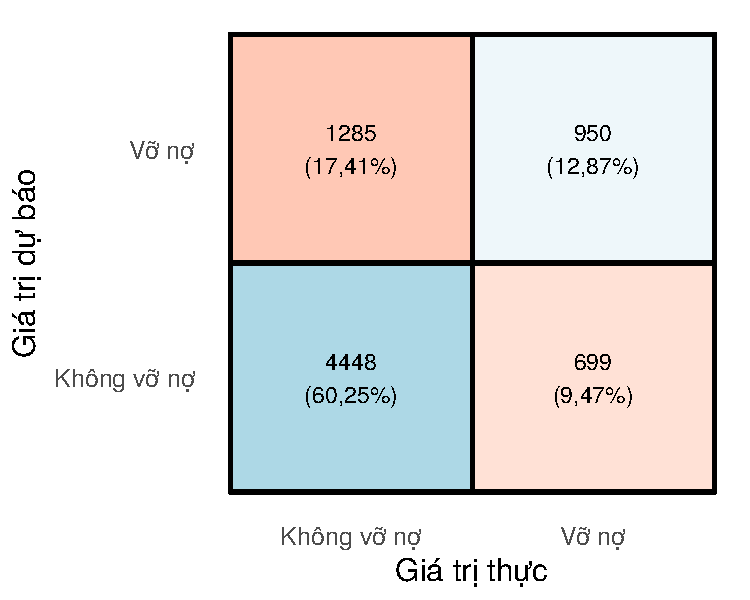
\includegraphics[width=10cm]{Figures/lasso_confusion_mat-1} 

\end{knitrout}
\caption{Confusion matrix cho mô hình Logit với điểm mức điểm phân loại vào nhóm vỡ nợ là \text{0,1117041}}
\label{fig:lasso_confusion_mat}
\end{figure}

So sánh ma trận ở Hình \ref{fig:lasso_confusion_mat} với ma trận ở Hình \ref{fig:svm_confution_mat}. Ta có thể thấy là với tỷ lệ dự báo các đối tượng thuộc nhóm vỡ nợ tương đồng ($12,87\%$), khả năng phân loại các khác hàng thuộc nhóm không vỡ nợ của mô hình Logit là thấp hẳn hơn so với mô hình SVM. Tỉ lệ đánh dấu nhầm các trường hợp không vỡ nợ của mô hình Logit là $17,65\%$, so với tỉ lệ $13,63\%$ của mô hình SVM.

Qua những phân tích ở trên chúng ta có thể rút ra các điêm khác biệt giữa hai mô hình Logit và SVM:
\begin{itemize}
  \item Mô hình Logit cho phép chúng ta ước lượng xác suất vỡ nợ phụ thuộc vào tác động của các biến trong mô hình. Các hệ số ước lượng của mô hình cũng là một cách để chúng ta rút ra được ý nghĩa của các biến số trong bộ số liệu lên xác suất vỡ nợ của khách hàng. Bằng cách sử dụng các giá trị cắt khác nhau, ta có thể điều chỉnh mức độ nhạy cảm của mô hình đối với việc phân loại các khách hàng xấu, phục vụ cho chính sách của ngân hàng.
  \item Mô hình SVM tuy không đưa ra một thang đo cụ thể cho các quan sát, nhưng lại là một mô hình có hiệu năng phân loại cao hơn, do quan hệ giữa các biến và khả năng vỡ nợ không bị ràng buộc bởi mô hình tuyến tính. Việc lựa chọn và ứng dụng các kernel và điều chỉnh các tham số của mô hình khiến cho mô hình rất linh hoạt, tuy nhiên lại làm cho ý nghĩa của các hệ số trong mô hình khó có thể diễn giải.
\end{itemize}

%%%%%%%%%%%% 
% Kết luận %
%%%%%%%%%%%%

\chapter{Kết luận}

%%%%%%%%%%%
% Phụ lục %
%%%%%%%%%%%
\appendix
\titlecontents{chapter}[0pt]{\bfseries}
  {\color{blue}PHỤ LỤC \thecontentslabel:\quad}
  {}{\titlerule*[1pc]{.}\contentspage}
  

\chapter{Thông tin về phiên làm việc trên R}

\begin{knitrout}\small
\definecolor{shadecolor}{rgb}{0.969, 0.969, 0.969}\color{fgcolor}\begin{kframe}


{\ttfamily\noindent\bfseries\color{errorcolor}{\#\# Error in system(paste(which, shQuote(names[i])), intern = TRUE, ignore.stderr = TRUE): cannot popen '/usr/bin/which 'uname' 2>/dev/null', probable reason 'Cannot allocate memory'}}\end{kframe}
\end{knitrout}

% \chapter{Code}




%%%%%%%%%%%%%%%%%%%%%%%
% Danh mục tham khảo  %
%%%%%%%%%%%%%%%%%%%%%%%
\printbibliography
\addcontentsline{toc}{chapter}{Tài liệu tham khảo}

\end{document}
